\documentclass[a4j,12pt,dvipdfmx]{jsreport}

% 数式
\usepackage{amsmath,amsfonts}
\usepackage{bm}

% 画像
\usepackage[dvipdfmx,top=35truemm,bottom=30truemm,left=30truemm,right=30truemm]{geometry}
\usepackage[dvipdfmx]{graphicx}
% biblatex
\usepackage[style=numeric, sorting=none, maxbibnames=1000]{biblatex}
\addbibresource{graduation_thesis.bib}

% itembox
\usepackage{ascmac}
% breakitemboxのためのpackage
\usepackage{itembkbx}
% \usepackage{tcolorbox} 画像が見えなくなってしまう原因
% \usepackage{framed} 枠

% フォント
\usepackage[ipaex]{pxchfon}
\listfiles
\usepackage{float}
\usepackage{multicol}
\usepackage{multirow}
\usepackage{paralist}
\usepackage{caption}
% \captionsetup{format=plain, justification=centering}
\usepackage{setspace}
\usepackage{algorithm}
\usepackage{algpseudocode}
\usepackage[dvipdfmx,hidelinks]{hyperref}
\usepackage{pxjahyper}
\usepackage{fancyhdr}
\usepackage{ltablex}
\usepackage{capt-of}
\usepackage{tabularx}
\usepackage[export]{adjustbox}
\usepackage{booktabs}
\usepackage{enumitem} % itemizeの行間 これは下になければならない
\usepackage{threeparttable} % 表の脚注
\usepackage{titlesec}
\usepackage{makecell}
\usepackage{forest}
\usepackage{fancybox}
% titlesec と \paragraph の相性問題を回避（run-in 見出しにする）
\titleformat{\paragraph}[runin]
  {\normalfont\normalsize\bfseries}
  {}{0pt}{} % ←ここには文字や \noindent 等を入れない
\titlespacing*{\paragraph}
  {0pt}{1.0ex}{0.8em}
\titleformat{\chapter}[hang]{\LARGE\bfseries}{\prechaptername\thechapter\postchaptername}{1em}{}

\setlength{\headheight}{16.5pt}
\captionsetup{format=hang}
\captionsetup[figure]{font=small}
\captionsetup[table]{font=small}
\begin{document}

% ▼▼▼ 仕掛け：main じゃないとき（単体のとき）だけヘッダー設定 ▼▼▼
\ifdefined\ismain\else
   \pagestyle{fancy}
   \lhead{\rightmark}
   \renewcommand{\chaptermark}[1]{\markboth{第\ \thechapter\ 章\ #1}{}}
   \setlength{\headheight}{16.5pt}
   \titleformat{\chapter}[hang]{\LARGE\bfseries}{\prechaptername\thechapter\postchaptername}{1em}{}
\fi
% ▲▲▲▲▲▲▲▲▲▲▲▲▲▲▲▲▲▲▲▲▲▲▲▲▲▲▲▲▲▲▲▲▲▲▲▲

\chapter{Manga109NameDataset}\label{chap:manga109name}

本章では，本研究の第二段階として構築した，
漫画ネームデータセット Manga109NameDataset について述べる．
本データセットは，漫画画像に紐づく脚本情報に加え，
詳細な演出情報を体系的に付与したものであり
物語から漫画作品へと至る過程を，
より高次な構造として捉えることを目的としている．

前章では，
Manga109ScriptDataset を用いた
脚本に基づく漫画レイアウト生成手法を検討し，
脚本情報が要素配置の精度や
ページ全体の幾何的一貫性に寄与することを示した．
しかし，序論で述べたとおり，
漫画制作におけるネームは，
単なる要素の配置結果ではなく，
視線誘導や強調，感情表現といった
演出上の意思決定が統合された，
より複合的な中間表現である．
そのため，
レイアウト生成のみを対象とした前章の設定では，
ネームが本来担う表現的側面を
十分に扱うことはできない．
本来の漫画制作におけるネームは，
作画に先立つ下書きとして描かれる視覚的な表現であるが，
本研究では，このネームを画像そのものとして直接扱うのではなく，
その中に含まれる本質的な設計要素を抽出し，
要素の幾何学的配置を表すレイアウト情報と，
演出上の意図を言語的に記述した演出情報とに分解する．
そして，これらを統合した構造化表現としてネームを定義する．
この抽象化は，
ネームが担う配置設計および演出上の意思決定を保持しつつ，
脚本からネーム生成へ至る過程を
計算機上で段階的に扱うための，
本研究における操作的定義である．

以上を踏まえ，本研究では，
近年のLVLMの性能向上を背景として，
漫画画像から脚本情報を改めて抽出し直すとともに，
キャラクターの振る舞いや表情，カメラワークといった
演出情報を新たに獲得し，
これらを構造的に整理した
Manga109NameDataset を構築した．
本研究では，このデータセットを，
後続章で扱う脚本に基づくネーム生成モデルの
学習および評価に適した基盤データとして位置づける．

本章の構成は以下の通りである．
まず~\ref{sec:name_overview} 節において，取り扱う演出情報に触れながら，
Manga109NameDataset の概要とそのデータ構造を説明する．
続いて~\ref{sec:name_construction} 節において，
データセットの構築にあたって整備した
読み順アノテーションおよび
独自のVisual Prompting の詳細，データセット構築の実行手順を説明する．
次に~\ref{sec:name_statistics} 節で，
構築したデータセットの統計量を示し，最後に~\ref{sec:name_sample} 節で構築したデータの可視化例を示す．

\section{Manga109NameDataset の概要}\label{sec:name_overview}
図\ref{fig:narrative_graph}に，
Manga109NameDataset における1サンプル分のデータ構造の概略を示す．
\begin{figure}[htbp]
   \centering
   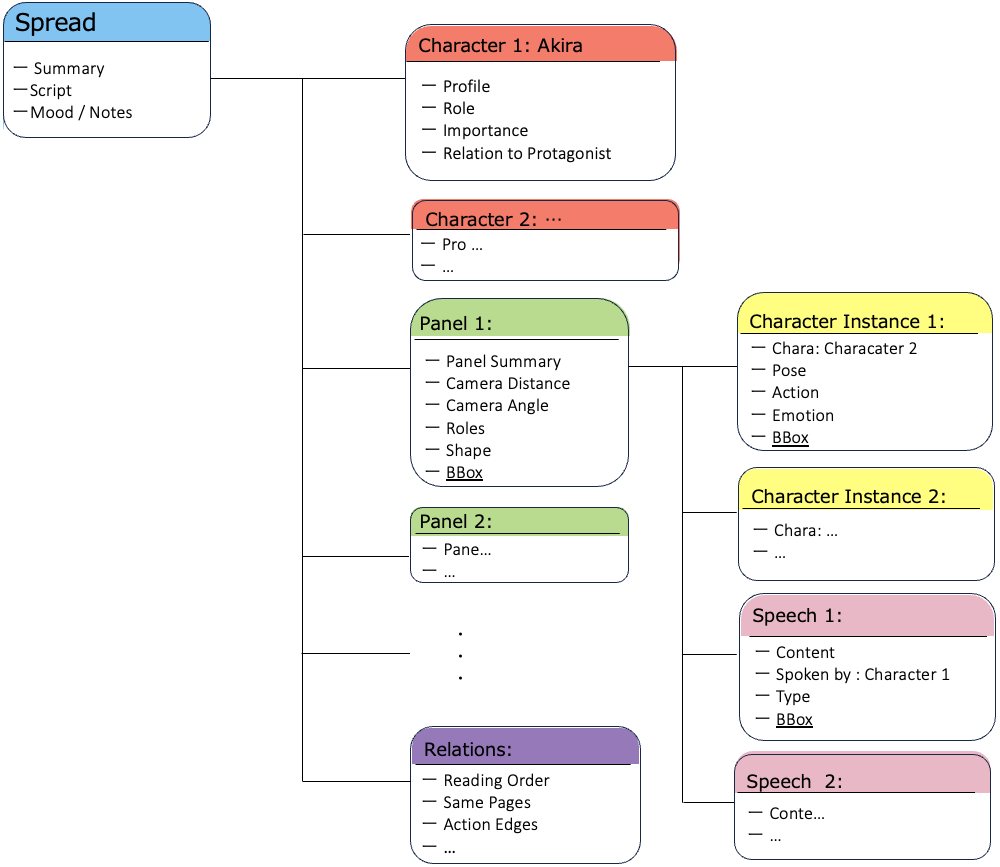
\includegraphics[width=\linewidth]{pict/05/narrative_graph.png}
   \caption{Manga109NameDataset における1サンプル分のデータ構造の概略}
   \label{fig:narrative_graph}
\end{figure}

Manga109NameDataset は，
漫画のネームを，
要素の幾何学的配置を表すレイアウト情報と，
脚本形式の記述を含む物語文章および演出情報を構造化したデータセットである．
本データセットでは，
漫画の見開きページ一つを基本単位とし，
その内部に含まれるコマ，キャラクター，セリフといった要素を
ノードとして定義するとともに，
それらの包含関係，参照関係，順序関係，および相互作用を
エッジとして明示的に表現する．
これにより，
ネームを構成要素と関係性の集合として捉え，
配置設計と演出上の意思決定を
計算機上で扱いやすい形式へと整理している．なお，見開き単位でデータを取得したのは，漫画の紙面構造上，見開きを一枚絵として捉え演出が設計されることが多いためである．

このように構成されたグラフにおいては，図\ref{fig:narrative_graph}に示すように
見開き全体に対応する \textbf{Spread ノード}を
物語および演出の文脈を担う最上位ノードとして位置づけている．
Spread ノードには，
当該場面の内容を要約した概要文や脚本記述，
場面全体の雰囲気や演出上の補足といった
グローバルな物語情報が付与される．
これらは，
配下に接続される各コマやキャラクター，セリフといった要素を，
個別の配置や表現としてではなく，
場面全体の流れや意図の中で解釈するための
上位文脈として機能する．

Spread ノードの下位には，
見開き内の各コマに対応する \textbf{Panel ノード}が配置される．
Panel ノードは，
漫画における最小の視覚的・演出的単位として，
物語の進行や演出上の役割を担う要素である．
各 Panel ノードには，
当該コマの内容を簡潔に記述した要約文に加え，
対話，反応，間（ま）といった物語上の役割，
コマ形状やカメラ距離・アングルといった
演出に関わる属性が付与される．
これにより，
コマ単体の意味内容と，
見開き全体における役割とを分離して記述することが可能となり，
レイアウト設計および演出制御の双方を
明示的に扱える構造となっている．

登場人物に関しては，
物語上の人物そのものを表す \textbf{Character ノード}と，
特定のコマ内に描かれた具体的な出現を表す
\textbf{Character Instance ノード}を分離して定義している．
Character ノードには，
人物名や性格，物語上の立ち位置といった
作品全体で共有される属性が付与される．
一方，
Character Instance ノードは，
特定のキャラクターの描写を表すノードであり，
姿勢，動作，感情といった
視覚的・演出的な具体像が記述される．
この分離により，
同一人物が複数のコマに異なる表情や振る舞いで登場する状況を，
構造的に自然な形で表現できる．

セリフは，
吹き出し単位で \textbf{Speech ノード}として管理される．
Speech ノードには，
発話内容のテキスト情報に加え，
発話の種類や，
どのキャラクター・どのコマに紐づくかといった
参照関係が付与される．
これにより，
言語表現と視覚要素との対応関係を
明示的に扱うことが可能となっている．

これらの各ノード間には，
包含関係，参照関係，順序関係，および相互作用を表す
複数種のエッジが定義されている．
これにより，
漫画ネームに内在する
空間的構造，時間的順序，および物語的関係性を，
単一のグラフ構造として統合的に表現している．また，直接的に紙面に描画される要素であるノード，Panel ノード，Character Instance ノード，Speech ノードには，バウンディングボックスの値を持たせ，レイアウト情報を表現している．

以上のように，Manga109NameDataset では，
見開き，コマ，キャラクター，セリフといった各要素を
グラフ上のノードとして整理し，
それぞれに対応する描画内容や場面における詳細な情報を集約することで，
漫画ネームに内在する演出上の意思決定を
構造化された形で表現している．
この構造により，
脚本に基づくネーム生成やレイアウト生成といった後続の処理において，
物語文脈，演出意図，および配置情報を
統合的に扱うことが可能となる．

\section{データセット構築手法}\label{sec:name_construction}
Manga109NameDataset の構築は，
Manga109ScriptDataset の構築と同様に，
LVLMを用いて漫画画像から必要な情報を抽出することを基本方針としている．
一方で，本データセットの構築では，
データの取得単位をページ単位ではなく見開き画像単位へと拡張し，
より高次な文脈および演出情報を扱う点で設定が異なる．
使用した LVLM は，
Gemini 3~\cite{woodward2025gemini3} および GPT-5.2~\cite{openai2025gpt52} であり，いずれも API を介して利用した．

漫画画像の読解における困難さについては，
Manga109ScriptDataset の構築過程において既に議論したとおりであり，
特に読み順の推定やキャラクターの識別は，
LVLM にとって依然として難しい課題である．
Manga109NameDataset の構築においても，
これらの問題は引き続き重要であり，
加えて見開き単位での処理に伴う
文脈の拡張や要素数の増加が新たな難点となる．

そこで本研究では，
ScriptDataset 構築時の知見を踏まえ，
読み順の明示的な付与や，
キャラクター識別を補助するための情報付加など，
複数の追加的工夫を導入することで，
これらの課題に対処した．
以下では，
Manga109NameDataset の構築に際して新たに導入した
各手法について順に説明する．

\subsection{読み順アノテーションの付与}\label{sec:reading_order_annotation}

漫画の内容理解において，
コマおよびセリフの読み順は，
物語構造を復元するための最も基本的な前提条件である．
Manga109ScriptDataset の構築においても，
読み順の推定が LVLM にとって困難であること，
既存手法による自動推定では誤りが残ることを確認している．
この問題は，
見開き単位で物語と演出を統合的に扱う
Manga109NameDataset においては，
より深刻な影響を及ぼす．

特に本データセットでは，
コマ間の時間的順序だけでなく，
セリフ間の発話順，
さらには演出上の「間（ま）」や反応の連なりを
正確に復元する必要がある．
そのため，
既存の自動推定結果や推論に依存するのではなく，
読み順を明示的な正解情報として与えることが不可欠であると判断した．

そこで本研究では，
Manga109Dataset に含まれる
全コマ 103{,}850 枚および
全セリフ 127{,}877 件に対して，
人手による読み順アノテーションを新たに付与した．
アノテーションは，
見開き内における読み進め順を基準として，
コマおよびセリフに一意な順序を割り当てる形で行った．

アノテーション作業にあたっては，
効率的かつ一貫した作業を行うため，
本研究独自のアノテーションツールを開発した．開発したツールを操作画面を図~\ref{fig:reading_order_tool} に示す．

\begin{figure}[htbp]
   \centering
   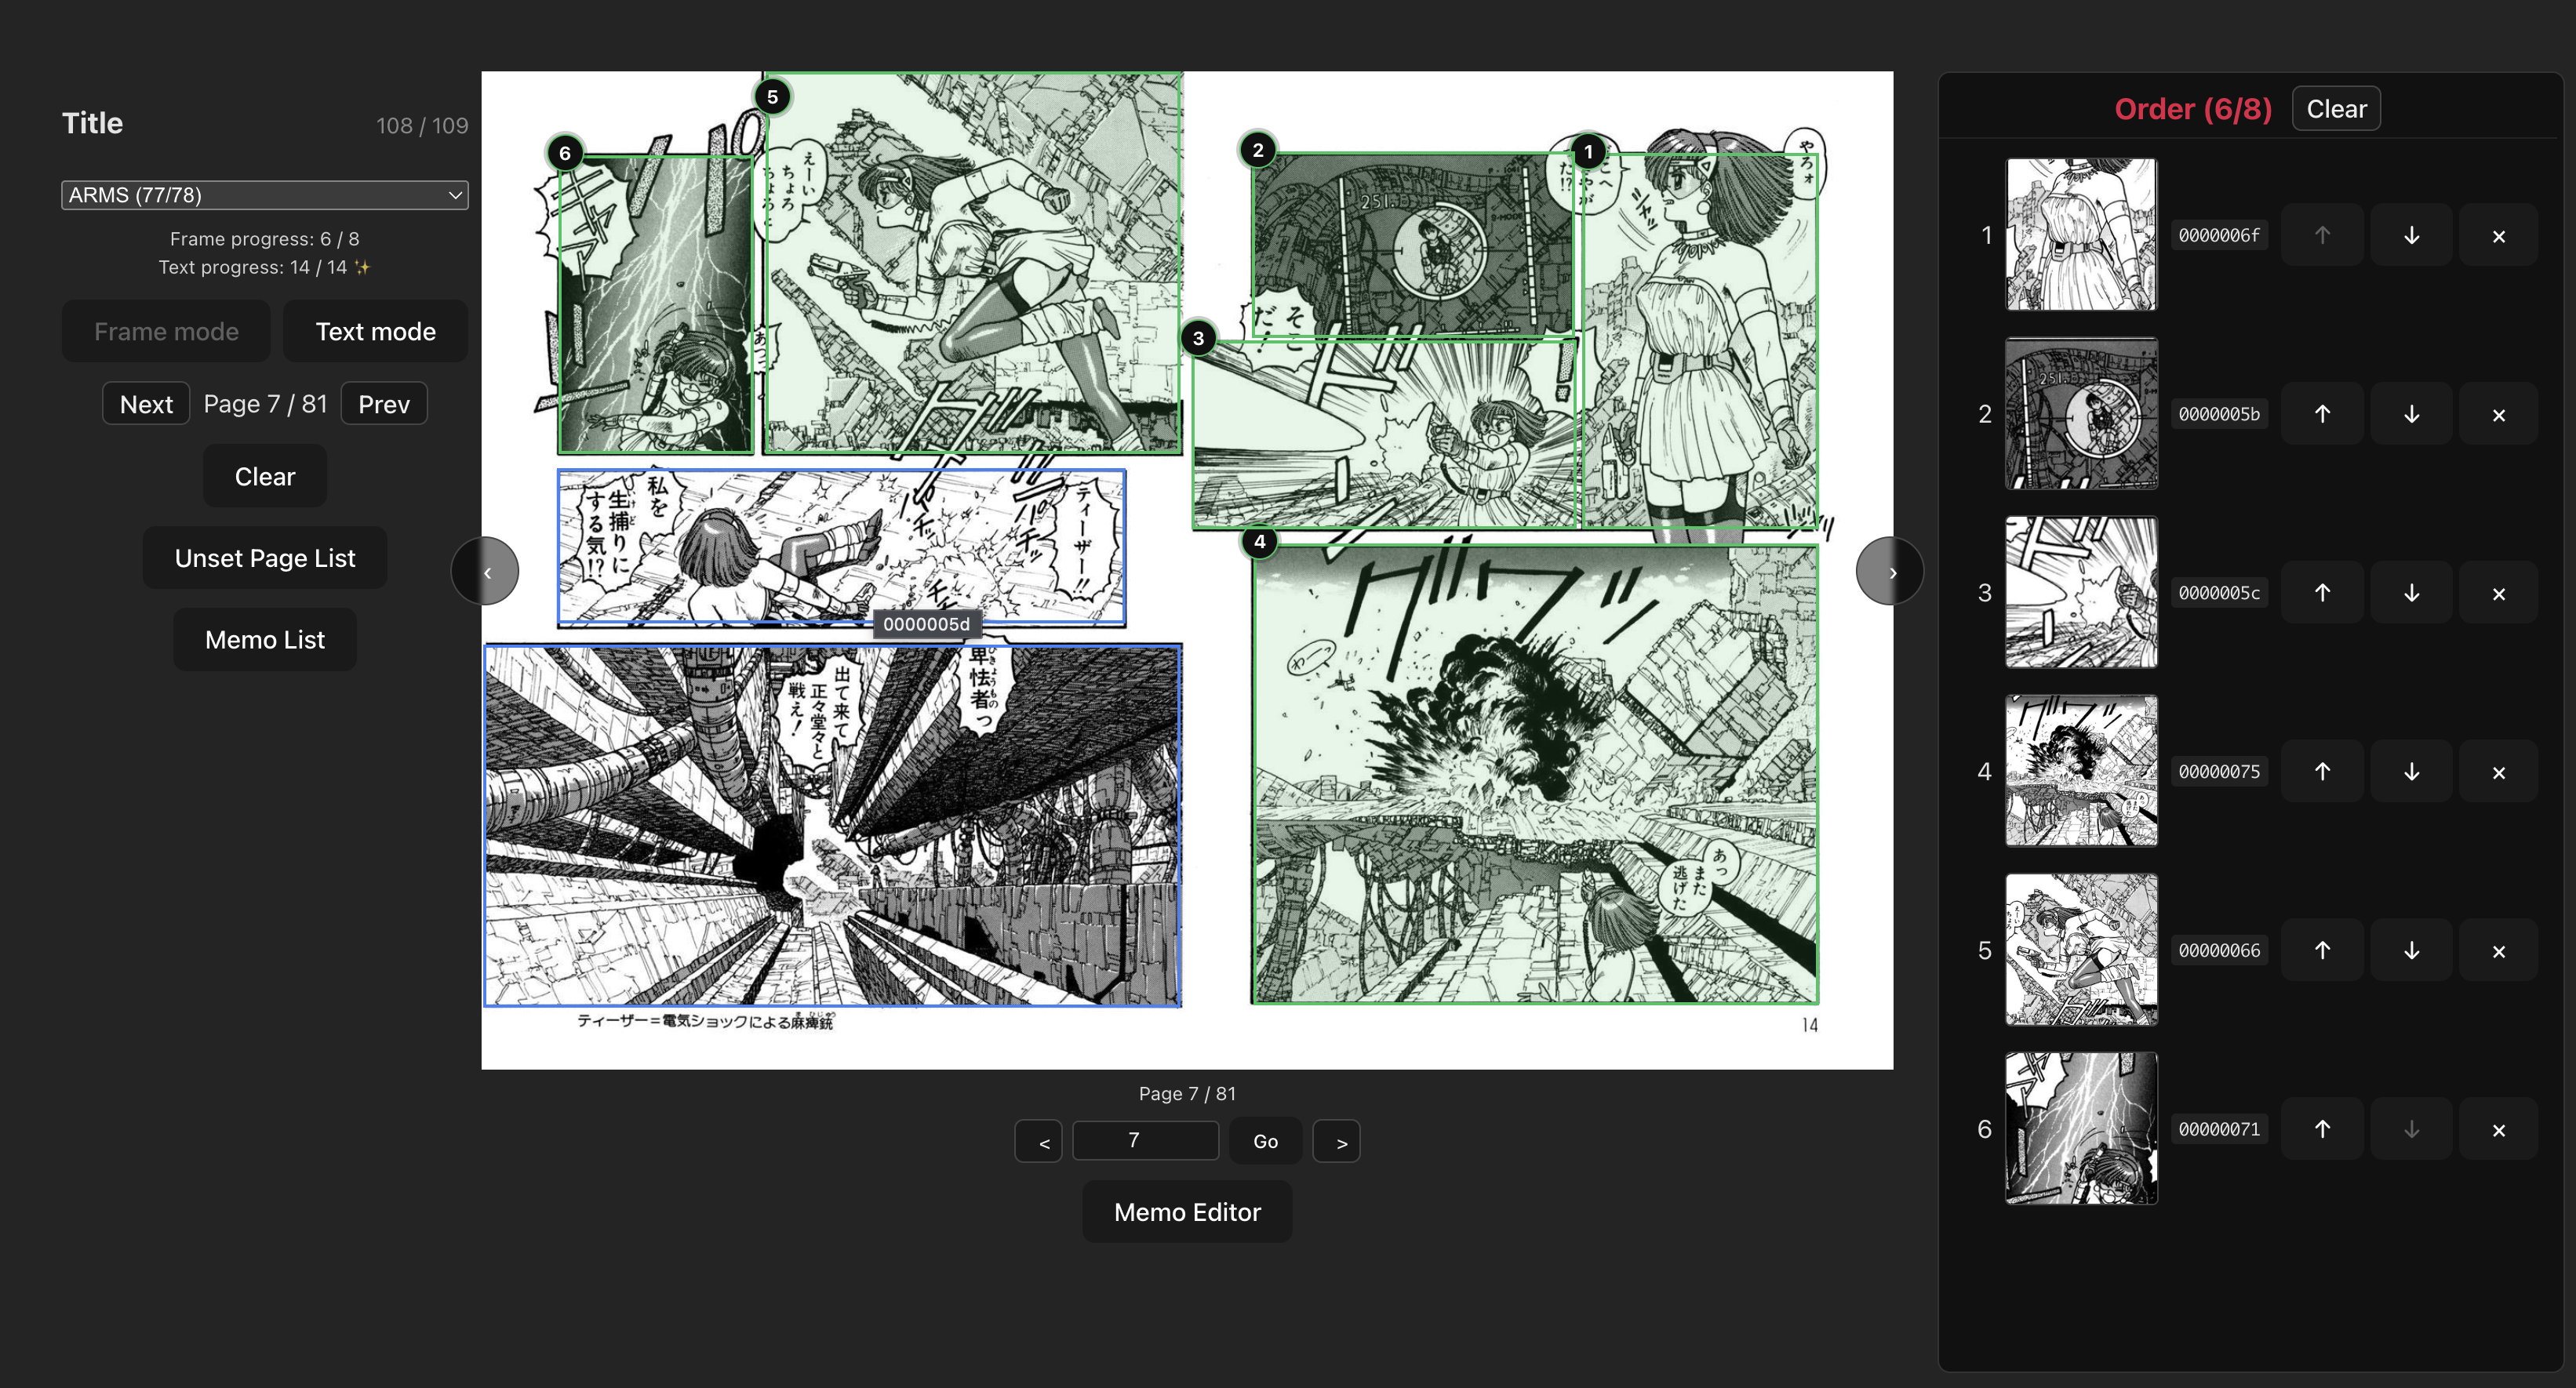
\includegraphics[width=\textwidth]{pict/05/reading_order_tool.png}
   \caption{読み順アノテーションツールの操作画面(漫画:『ARMS』©加藤 雅基/東京三世社)}
   \label{fig:reading_order_tool}
\end{figure}

本ツールでは，
見開き画像を表示しながら，
コマおよびセリフを選択し，
直感的に順序を指定できるインタフェースを備えている．
実作業は，
筆者が中心となって進めるとともに，
一部については産業技術総合研究所の技術支援者の協力を得て実施した．

このようにして付与された読み順アノテーションは，
後述するビジュアルプロンプティングにおいて
LVLM に与える重要な手がかりとして利用されるほか，
データセット全体の構造的整合性を保証する基盤情報として機能する．

\paragraph{既存手法との読み順の差異}
読み順推定手法として知られる Manga Whisperer~\cite{sachdeva_manga_2024-1}のアルゴリズムについて，
本研究では，
人手アノテーションとの順序一致率を比較評価した．
その結果，
見開き画像単位で順序が完全一致しなかった割合は，
コマについて 1{,}121 / 10{,}122（11.87\%），
セリフについて 2{,}609 / 10{,}043（25.98\%）であった．
本研究では，
コマ単位やセリフ単位での部分的な誤りの定義が困難であることから，
順序が完全一致しなかった見開き画像の割合を指標としている．

図~\ref{fig:reading_order_diff1}，~\ref{fig:reading_order_diff2} に，
それぞれコマとセリフの読み順が一致しなかった見開き画像の例を示す．


\begin{figure}[htbp]
   \centering
   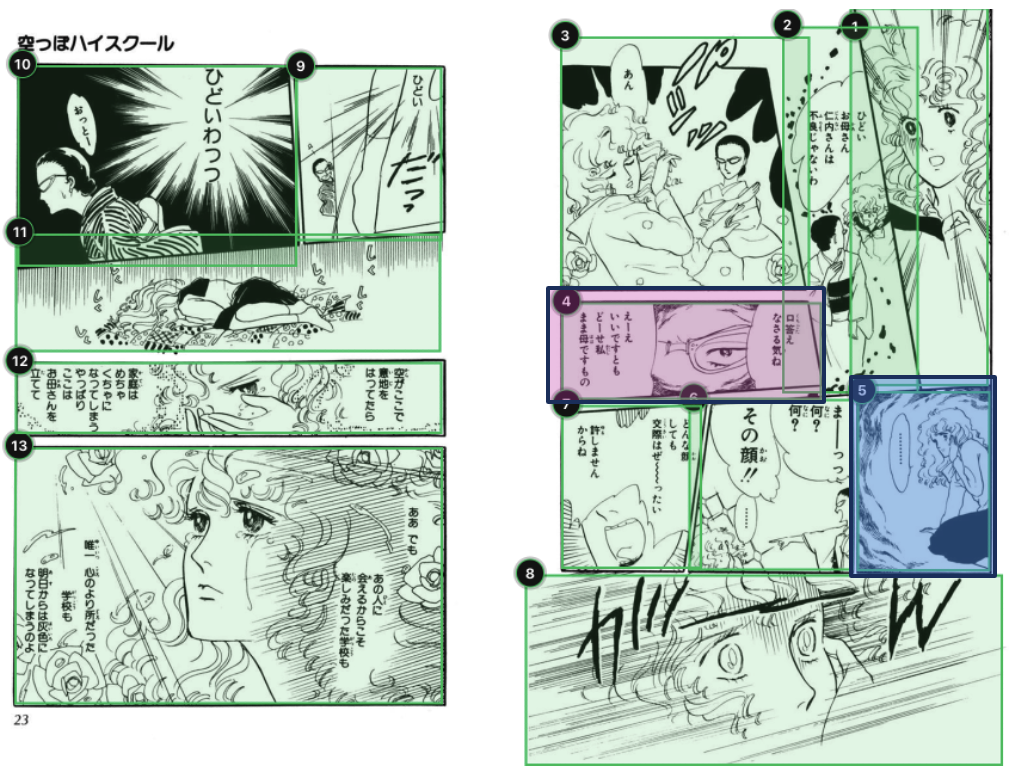
\includegraphics[width=\textwidth]{pict/05/reading_order_diff1.png}
   \caption{コマの読み順が一致しなかった見開き画像の例．本来は4，5と読み進めるべきコマの順序が，自動推定では逆転してしまった(漫画:『空っぽハイスクール』©	高口 里純/角川書店)．}\label{fig:reading_order_diff1}
\end{figure}

コマの読み順について，
Magi による自動推定が正しく行えなかった事例を分析した結果，
図~\ref{fig:reading_order_diff1} に示すように，
長方形近似に基づく配置推定の影響や，
左上と右下に配置されたコマ同士の比較において
内容理解を要する場合，
さらに吹き出しによる視線誘導が
コマの幾何学的配置による優先順位を凌駕する場合などが確認された．
これらの事例では，
単純な空間配置に基づく規則のみでは，
実際の読解順を適切に復元できないことが分かる．


\begin{figure}[htbp]
   \centering
   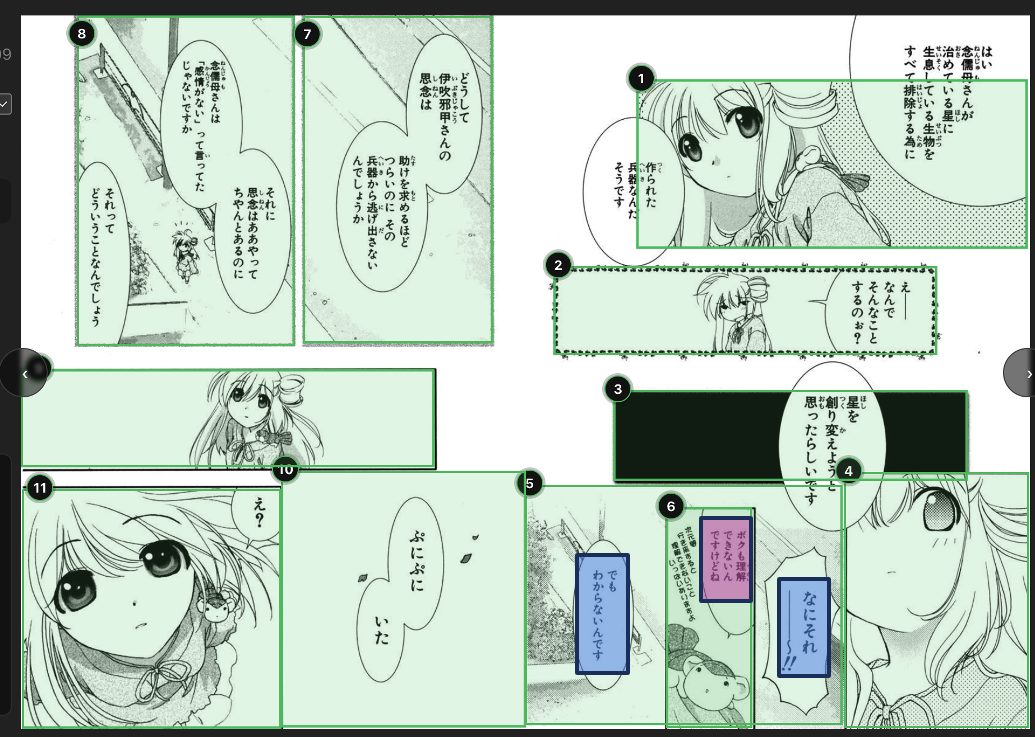
\includegraphics[width=\textwidth]{pict/05/reading_order_diff2.png}
   \caption{セリフの読み順が一致しなかった見開き画像の例．本来は6番のコマに帰属するセリフは，5番のコマに帰属する２つのセリフの間で読まれるべきであるが，自動推定では5番のコマの２つのセリフよりも後に推定されてしまった(漫画:『ヒーリング・プラネット』©桜野 みねね/	エニックス)．}\label{fig:reading_order_diff2}
\end{figure}

一方，セリフの読み順についても，
自動推定が困難となる特徴的な状況が観察された．
具体的には，図~\ref{fig:reading_order_diff2} に示したような
セリフの順序が帰属するコマの順序に強く制約される場合や，
本来的に明確な帰属先コマを持たない
「宙に浮いた」セリフが存在する場合である．
後者のようなケースでは，
アルゴリズム上，
最も近傍のコマに機械的に割り当てられることで
順序が決定されるため，
実際の読解順と乖離が生じやすい．
また，
左上と右下に配置されたセリフ同士の順序関係は
セリフ内容の意味理解に依存する場合も確認された．

以上の分析から，
漫画における読み順は，
コマ配置，吹き出しによる視線誘導，
内容理解，演出的意図といった
複数の要因が複合的に関与して決定されることが多く，
その自動推定は本質的に困難な課題であることが明らかとなった．
本研究では，
これらの問題に対処するため，
人手により付与した読み順アノテーションを
正解情報として利用し，
後続のデータ取得および LVLM による読解性能の基準として用いている．

\subsection{ID 情報を付記する独自 Visual Prompting}\label{sec:visual_prompting_with_id}

本研究では，
付与した読み順アノテーションを
LVLM による漫画理解および情報抽出に
効果的に反映させるため，
コマおよびセリフに一意な ID を付与し，
それを視覚的に画像上へ埋め込む
独自の Visual Prompting 手法を導入した．図~\ref{fig:visual_prompting_with_id}に実際に使用した Visual Prompting の例を示す．

\begin{figure}[htbp]
   \centering
   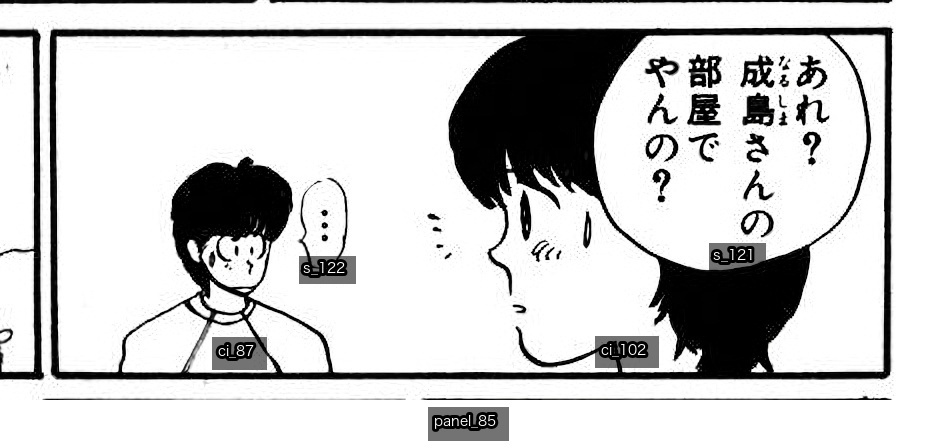
\includegraphics[width=\textwidth]{pict/05/id_visualprompting.jpg}
   \caption{IDを付記したVisual Prompting の例(漫画:『愛さずにはいられない』©よし まさこ/集英社)．}
   \label{fig:visual_prompting_with_id}
\end{figure}

Manga109ScriptDataset の構築においては，
ページ単位で漫画画像を入力し，
そのページ全体に対応する脚本を
一つのテキストとして生成すれば十分であった．
そのため，
生成された脚本と
画像内の個々のコマやセリフとの
厳密な対応関係を
明示的に管理する必要はなかった．

これに対し，
Manga109NameDataset では，
見開き内に含まれる
各コマ，各キャラクター，各セリフといった
描画要素ごとに，
演出情報や構造的な属性を
個別に抽出・整理することを目的としている．
すなわち，
本データセットの構築では，
「見開き全体から一つの脚本を得る」のではなく，
「見開き内の各描画要素から
それぞれに対応する情報を取得する」
という，より細粒度な対応付けが必要となる．

このような設定では，
LVLM が生成した記述と，
元画像上の具体的なコマやセリフ，
さらにはキャラクターの出現とを
正確に対応付けることが不可欠である．
しかし，
画像内に多数の要素が混在する漫画表現において，
自然言語による参照や
位置関係の暗黙的な推論のみに依存すると，
対応関係が曖昧になりやすい．

そこで本研究では，
読み順アノテーションに基づき，
各コマおよび各セリフに
連番の ID を付与するとともに，
これらの ID を
漫画画像上に直接描画した画像を
LVLM への入力として用いた．
具体的には，
見開き画像全体に加え，
各コマを個別に切り出した画像を
読み順に従って入力し，
それぞれの画像内に
対応するコマ ID やセリフ ID を
明示的に表示した．ID の表示は描画対象の画像領域に対する6\%の面積を占める小さな枠内に配置し，小さくなりすぎて認識されなくなることを防ぐため，最小フォントサイズを 12pt に設定した．

この ID 表示は，
単なるデータ管理上の識別子ではなく，
LVLM に対して
「どの要素を指しているのか」を
視覚的にアンカーする役割を果たす．
これにより，
生成される脚本記述や演出情報を，
特定のコマやセリフ，
さらにはキャラクターの具体的な出現と
一対一に対応付けることが可能となった．
また，
ID を介した参照により，
キャラクター名の誤同定や，
セリフと話者の取り違えといった
問題の発生を大きく抑制できることを確認している．

さらに，
画像入力の構成についても工夫を行った．
近年の LVLM においては
入力可能なトークン数が大幅に増加していることから，
本研究では，
対象とする見開き画像に加え，
当該見開き内の全コマを
個別画像として切り出し，
読み順に並べて入力する方式を採用した．
この際，
ID 表示は各コマ画像側に付与し，
見開き全体像と局所的な詳細情報とを
同時に参照できる構成とした．

このような
ID 情報を視覚的に付与する Visual Prompting により，
LVLM は，
漫画における空間配置と読み順，
物語的な対応関係，キャラクター識別を
より安定して理解できるようになり，
これはネーム構造の抽出精度向上に
大きく寄与した．

図~\ref{fig:panel_json_structure_with_id} に，付記した ID により，キャラクターの識別及び状況の理解が適切に行われた生成結果の例を示す．


\begin{figure}[htbp]
   \centering
   % 全体のレイアウト：左右に分割
   \begin{tabular}{@{}p{0.40\linewidth}@{\hspace{1em}}p{0.56\linewidth}@{}}
      % --- 左側：画像 ---
      % 画像内のID (s_12, ci_7など) が見えるように配置
      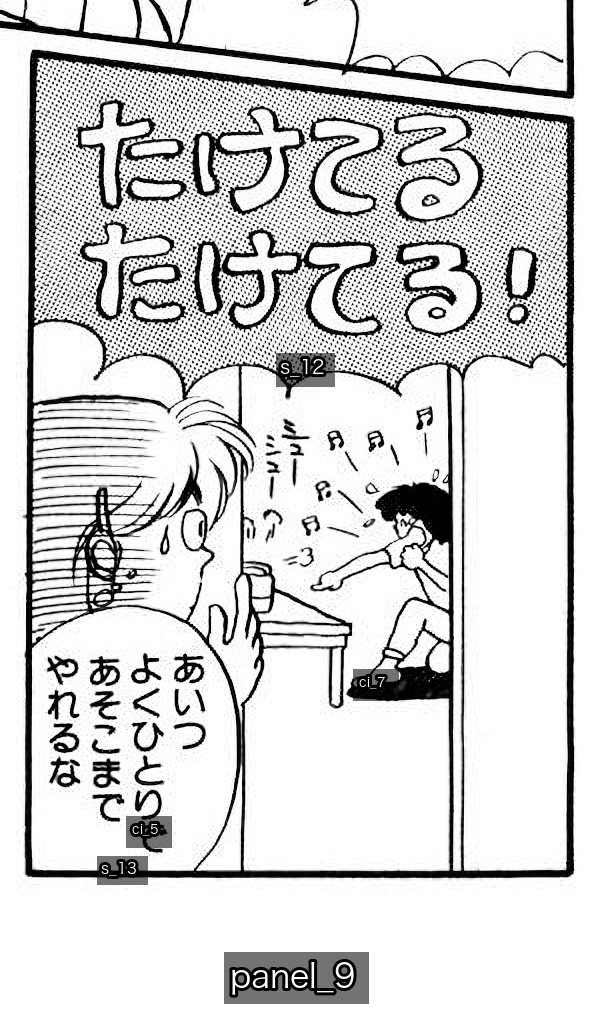
\includegraphics[width=\linewidth, valign=t]{pict/05/13_panel_panel_9.jpg}
       &
      % --- 右側：ID対応表 ---
      \small
      \adjustbox{valign=t}{%
         \renewcommand{\arraystretch}{1.35} % 日本語のために行間を少し広めにする
         % 左列(項目)は最小幅、右列(値)は折り返しあり
         \begin{tabular}{@{}l p{0.65\linewidth}@{}}
            \toprule
            \textbf{Attribute} & \textbf{Value / Description}                                               \\
            \midrule

            % --- Narrative Context (物語内容) ---
            \multicolumn{2}{@{}l}{\textit{\textbf{Narrative Context}}}                                      \\
            \quad ID           & \texttt{panel\_9}                                                          \\
            \quad Summary      & ご飯が炊けたことを踊って祝うあゆみと，それをドアの陰から見ているあさみ．                                       \\
            \quad Emotion      & \textbf{Joy} (あゆみ) vs \textbf{Confusion} (あさみ)                             \\

            % --- Cinematic (映像演出) ---
            \midrule
            \multicolumn{2}{@{}l}{\textit{\textbf{Cinematic \& Visuals}}}                                   \\
            \quad Shot         & Long Shot (LS), Eye-level                                                  \\
            \quad Composition  & 手前のあさみから，奥のあゆみへの視線誘導（Split depth）                                          \\

            % --- Graph Structure (IDによる構造化) ---
            % ここでIDを強調し、画像とのリンクを示す
            \midrule
            \multicolumn{2}{@{}l}{\textit{\textbf{Graph Structure (w/ IDs)}}}                               \\
            \quad Characters   & \texttt{ci\_7}: あゆみ (Dancing) \par \texttt{ci\_5}: あさみ (Watching)          \\
            \quad Speech       & \texttt{s\_12}: 歌唱・チャント (あゆみ) \par \texttt{s\_13}: 思考 (あさみ)                \\
            \quad Action Edge  & \texttt{ci\_5} (あさみ) $\xrightarrow{\text{observing}}$ \texttt{ci\_7} (あゆみ) \\

            \bottomrule
         \end{tabular}%
      }
   \end{tabular}

   \caption{IDラベルによりキャラクターの識別等状況が正確に構造化された例．画像内のIDタグである \texttt{ci} (Character Instance) はキャラクターを，\texttt{s} (Speech) はセリフを一意に識別しており，これらが右側の構造化データとして正しく対応付けられている(漫画:『愛さずにはいられない』©よし まさこ/集英社)．}
   \label{fig:panel_json_structure_with_id}
\end{figure}

\subsection{超解像度処理による認識性能の向上}\label{sec:super_resolution}

漫画画像には，
小さなコマや細密な描写が多く含まれており，
LVLM による内容理解において，
視認性の低さが性能低下の一因となる．
特に本研究では，
コマやセリフに ID ラベルを付記した画像を
入力として用いるため，
これらのラベルが
本来の描画内容を遮蔽し，かえって
視覚的理解を妨げるオクルージョンの問題が生じる．
そこで本研究では，
小さなコマの理解精度向上と，
ID ラベルによる視認性低下の抑制を目的として，
漫画画像に対する超解像度処理を導入した．

具体的には，
オープンソースの超解像モデルである
DRCT~\cite{DRCT} を用い，
元画像に対して
$\times 4$ の超解像処理を施した．
これにより，
細部の線画や文字情報が明瞭化され
LVLM による視覚的理解の安定化と，また ID が付記できるスペースを生み Visual Prompting の効果を高めることが可能となった．例えば，オクルージョンの問題を解決する手段としては，単純にフォントサイズを画像比率にあわせ縮小する方法も考えられるが，コマ画像のサイズによっては，描画できる最小フォントサイズに満たない場合もしばしば存在した．図~\ref{fig:super_resolution}に示すように，超解像度処理を施すことでこのような画像に対しても適度なサイズで ID ラベルを描画することが可能となった。

\begin{figure}[htbp]
   \centering
   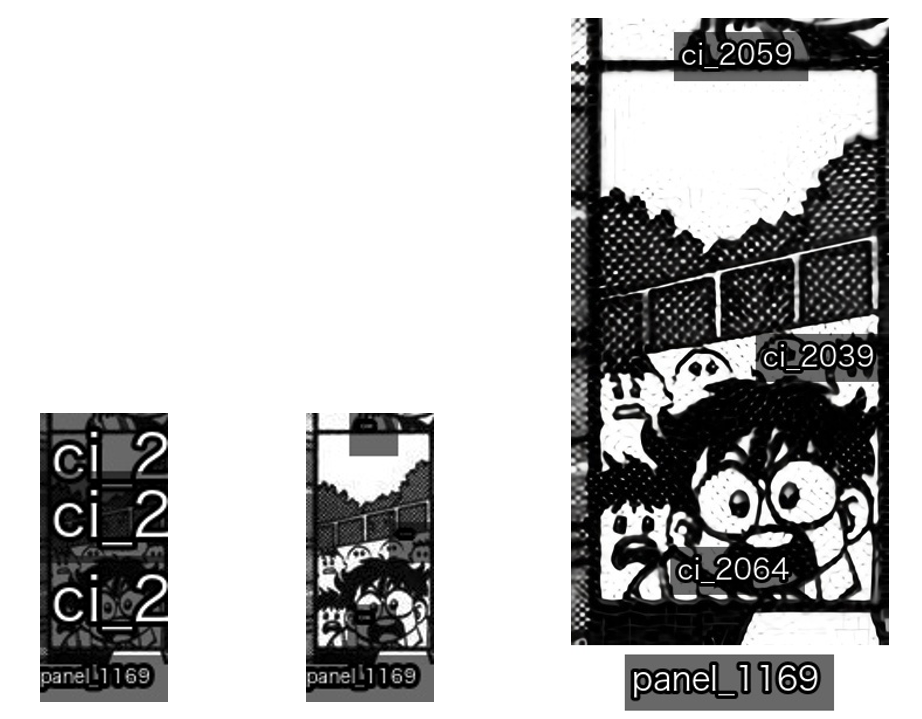
\includegraphics[width=0.5\textwidth]{pict/05/super_resolution.png}

   \caption{超解像度処理によるIDラベルの視認性が向上した例．左が最小フォントサイズを12ptに設定した画像，中央が画像比率にあわせ最小フォントサイズを設定した画像，右が超解像度処理を施し12ptのフォントサイズを設定した画像である．左は画像全体にオクルージョンが生じ，中央はラベル自体が付記できていないが，右は適度なサイズでIDラベルを描画できている(漫画:『うるとら★イレブン』©やぶの てんや, 渡辺 達也/集英社)．}
   \label{fig:super_resolution}
\end{figure}



一方で，
単純に高解像度化した画像を
そのまま LVLM に入力すると，
API の入力制約やタイル分割方式の影響により，
通常の画像であれば認識可能である
12pt 程度のフォントサイズであっても，
相対的に埋め込み領域が狭くなり，
ID ラベルが正しく認識されなくなる
問題が確認された．

この問題に対処するため，
本研究では，
$\times 4$ の超解像画像に対して，
線形輝度空間へ変換した上で
平均化処理を伴うダウンサンプリングを行い，
解像度を $\times \frac{1}{2}$ に縮小する手法も採用した．
この処理により，
元画像比で $\times 2$ 相当の解像度を持つ画像を生成し，
元画像の大きさや ID ラベルのサイズに応じて，
最も認識精度が高くなる
超解像度設定を選択できるようにした．

具体的な運用条件としては，
LVLM の API における1タイルが512×512ピクセルである
タイル分割方式を考慮し，
各コマ画像の超解像度化後の画像が
最大 4 タイル内で処理可能となるよう
画像サイズを調整した．
この条件下において，
ID ラベルの最小フォントサイズを
12pt 以上に維持しつつ，
描画内容へのオクルージョンが
最も小さくなる
超解像度設定および
入力コマ画像の選択を行った．

図\ref{fig:super_resolution_box}に，IDラベルの最小フォントサイズの縮小に伴う遮蔽率の変化と超解像度処理に伴う遮蔽率の比較を示す．これより，フォントサイズのを縮小する操作に比べると，2倍の超解像度処理でさえ、十分に遮蔽率の低減に優れた効果があることがわかる．

\begin{figure}[h]
   \centering
   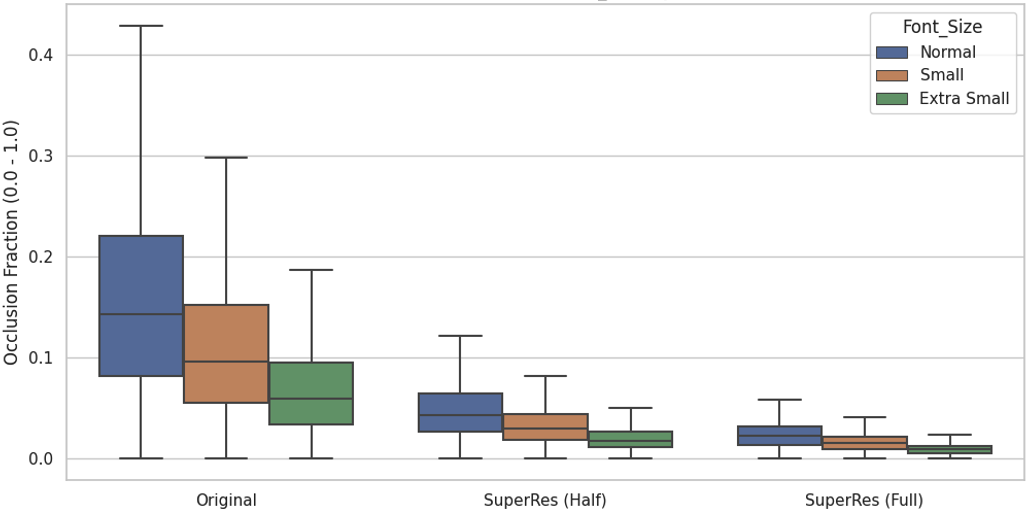
\includegraphics[width=\textwidth]{pict/05/super_resolution_box.png}

   \caption{IDラベルの最小フォントサイズの縮小に伴う遮蔽率の変化と超解像度処理に伴う遮蔽率の比較．Normal の最小フォントサイズは12ptで設定され，Small は9pt，Extra Small は6ptに設定された．SuperRes(Half)は２倍の超解像度処理画像，SuperRes(Full)は4倍の超解像度処理画像を表す．}
   \label{fig:super_resolution_box}
\end{figure}


以上の超解像度処理により，
小さなコマや細部表現の可読性が向上するとともに，
ID ラベルの付記が
漫画内容の理解を妨げる影響を
効果的に抑制できた．
この処理は，
後続の LVLM による
演出情報およびネーム構造の抽出を
安定して行うための
重要な前処理として機能している．

\subsection{文脈理解を促進する画像・セリフの入力}\label{sec:contextual_input}

漫画における演出や物語理解は，
単一の見開きやコマの内容のみから
完結するとは限らない．
特に，
キャラクターの関係性や感情の変化，
ギャグや伏線といった表現は，
前後の展開を踏まえて初めて
正しく解釈される場合が多い．
そのため，
対象とする見開き画像のみを
LVLM に入力した場合，
文脈依存の表現に対して
誤った解釈や表層的な記述が
生成されることが確認された．

そこで本研究では，
対象見開きに関する情報抽出に先立ち，
当該場面の前後文脈を
LVLM に明示的に与えることで，
漫画全体の流れを踏まえた理解を
促進する入力構成を採用した．
具体的には，
対象とする見開き画像に加え，
過去 9 ページ分の見開き画像，
および次の 1 ページ分の見開き画像を
併せて入力として与えた．
これにより，
直前までの展開や，
次に起こる反応を含めた
時間的連続性を
視覚的に参照可能とした．

さらに，
視覚情報だけでなく，
テキスト情報としても
物語文脈を補強するため，
過去ページに含まれる
全セリフを，
付与済みの読み順アノテーションに基づいて
正しい順序で入力した．
加えて，
それらのセリフ内容を
LVLM に要約させたテキストを併用し，
長距離文脈を簡潔に保持できるようにした．
この要約は，
対象見開きに至るまでの
物語状況やキャラクター関係を
高次の文脈として与える役割を果たす．

このように，
見開き画像，
個別コマ画像，
過去・未来ページの視覚情報，
および読み順付きセリフとその要約を
組み合わせて入力することで，
LVLM は，
単一ページに閉じた解釈ではなく，
物語全体の流れを踏まえた理解を
行えるようになる．
実際に，
対象見開きの概要文（Spread summary）には，
前段の出来事を前提とした記述や，
キャラクターの感情的変化を反映した表現が
含まれるようになり，
キャラクター名の誤同定や
関係性の取り違えも
大きく減少することを確認している．

以上の文脈情報を付与した入力構成は，
後続の演出情報および
ネーム構造の抽出において，
場面理解の一貫性と
記述の安定性を高める上で
重要な役割を果たしている．

図\ref{fig:contextual_summary_example}は，
文脈付与入力により，
見開き単体では読解困難な，過去のシーンの状況の理解が必要な場面で生成された概要分の抜粋を示す．このシーンでは，過去に登場した田中重夫という呼称に理解がないと読解できないが，文脈付与入力により正しく状況を理解することができている．

\begin{figure}[htbp]
   \centering
   \begin{tabular}{@{}p{0.48\linewidth}@{\hspace{1em}}p{0.48\linewidth}@{}}
      % --- 左側：画像 ---
      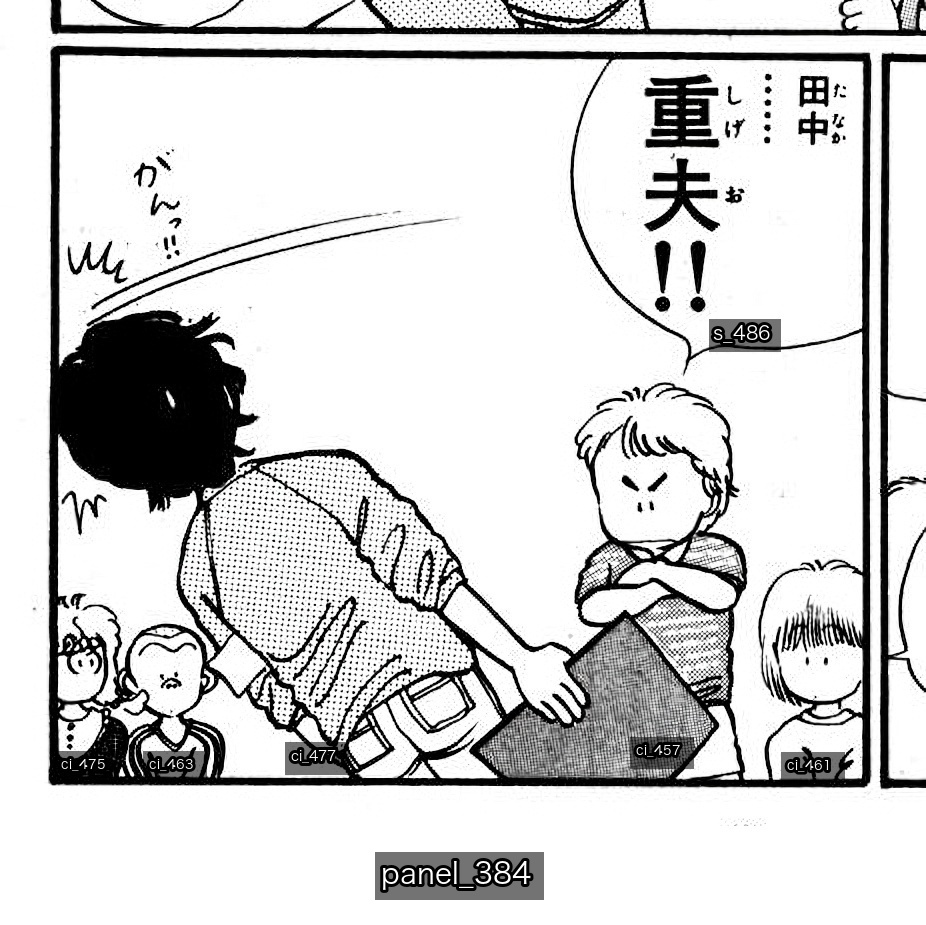
\includegraphics[width=\linewidth, valign=t]{pict/05/context_example.jpg}
       &
      % --- 右側：テキストボックス ---
      % ▼ ここでローカル設定（この図だけに適用）
      {
            \setlength{\fboxsep}{5mm} % 枠と文字の隙間を5mmに広げる（重要）
            \cornersize{0.3}          % 角の丸み具合
            \adjustbox{valign=t}{%
               \ovalbox{%
                  % 幅の計算は \fboxsep の変更に合わせて自動調整されます
                  \begin{minipage}[t]{\dimexpr\linewidth-2\fboxsep-2\fboxrule\relax}
                     \small
                     \linespread{0.75}\selectfont % 行間を広げて読みやすくする（モダン化）

                     \textbf{生成された summary の抜粋}\\[6pt]

                     「名前をいいなさい」と告げた。重夫は
                     「くっそお、きったねーっ！！」と
                     悔しがりながらも、観念したように
                     大声で叫んだ。
                     「ほれ！！名前」「田中……重夫！！」。
                     その名前を聞いた瞬間、歩の頭に衝撃が走る。
                     大家さんがいつも自分を呼ぶあの名前と
                     同じだったのだ。
                  \end{minipage}%
               }%
            }
         }
   \end{tabular}

   \caption{文脈付与入力により，見開き単体では理解が困難な場面で，過去の状況を正しく盛り込み正確な理解で summary が生成された例(漫画:『愛さずにはいられない』©よし まさこ/集英社)．}
   \label{fig:contextual_summary_example}
\end{figure}

\section{Manga109NameDataset の統計的特性}
\label{sec:name_statistics}

本節では，構築した
Manga109NameDataset の規模および構成要素の分布について，
各ノード種別および付与した属性の統計量を示す．以下では，
まずデータセット全体の規模を示し，
続いて各ノードに付与された情報の分布について，
ノード種別ごとに詳細を述べる．

\subsection{データセット全体の規模}
\label{sec:dataset_overview_stats}

表~\ref{tab:dataset_overview} に，
Manga109NameDataset に含まれる
見開き（Spread）ノード数，
および各ノード種別の総数と，
1 Spread あたりの平均数を示す．

\begin{table}[htbp]
   \centering
   \caption{Manga109NameDataset に含まれる各ノード種別の総数と 1 Spread あたりの平均数．なお Characterノードについても Spread ごとに集計した数を示す．}
   \label{tab:dataset_overview}
   \begin{tabular}{lrrrr}
      \hline
      \textbf{ノード種別}     & \textbf{総数} & \textbf{平均} \\
      \hline
      Spread             & 9{,}827     & 1.00        \\
      Panel              & 102{,}600   & 10.44       \\
      Character          & 39{,}478    & 4.02        \\
      Character Instance & 153{,}844   & 15.66       \\
      Speech             & 144{,}875   & 14.75       \\
      \hline
   \end{tabular}
\end{table}

表~\ref{tab:dataset_overview}に示された通り，本データセットは，Manga109Datasetに含まれる全見開き画像のうち，内部にコマ(Panel)を有するすべての画像を対象に構築されており，
合計 9{,}827 見開き分のデータを含む．
Manga109Datasetに含まれるすべてのコマの数は，全103,850コマであり，本データセットの構築においては，その98.8\%のコマに対して情報が抽出されたことを確認した．

\subsection{Spread ノードに付与された物語情報の統計}
\label{sec:spread_node_stats}
表~\ref{tab:spread_summary_stats} に，
Spread ノードに付与された
概要文（summary）の文字数分布に関する
統計量を示す．

\begin{table}[htbp]
   \centering
   \caption{Spread ノードに付与された summary の文字数の統計．}
   \label{tab:spread_summary_stats}
   \begin{tabular}{lr}
      \toprule
      \textbf{項目} & \textbf{数値} \\
      \midrule
      Spreadの総数   & 9{,}827     \\
      \cmidrule(lr){1-2}
      平均文字数       & 112.81      \\
      中央値文字数      & 94.00       \\
      最小文字数       & 12          \\
      最大文字数       & 702         \\
      標準偏差        & 79.07       \\
      \bottomrule
   \end{tabular}
\end{table}
平均で約 110 文字程度の概要文が付与されており，
見開き単位での物語内容や文脈を
簡潔かつ情報量を保った形で記述できていることを確認した．

\subsection{Panel ノードに付与された構成要素と演出属性の統計}
次に，Panel ノードに付与された構成要素と演出属性の統計を示す．

\paragraph{Panelのsummaryの文字数統計}
\label{sec:panel_summary_stats}
表~\ref{tab:panel_summary_stats} に，
Panel ノードに付与された概要文（summary）の
文字数統計を示す．summary は，各コマの視覚内容を簡潔に言語化したものであり，
大多数のコマに対して付与されている．

\begin{table}[htbp]
   \centering
   \caption{Panel ノードに付与された summary の文字数統計．}
   \label{tab:panel_summary_stats}
   \begin{tabular}{lr}
      \toprule
      \textbf{項目} & \textbf{数値} \\
      \midrule
      Panelの総数    & 102{,}600   \\
      \cmidrule(lr){1-2}
      平均文字数       & 79.20       \\
      中央値文字数      & 81.00       \\
      最小文字数       & 0           \\
      最大文字数       & 326         \\
      標準偏差        & 37.44       \\
      \bottomrule
   \end{tabular}
\end{table}

summary の文字数が 0 となったコマは，
全体の 2{,}058 / 102{,}600 コマ（約 2.01\%）に相当する．
これらの多くは，間（ま）やリズムを演出することを主目的とした
装飾的・演出的性格の強い空白コマであり，
その内容自体には summary として記述すべきものが見られないコマであった．平均すると約 79 文字程度の
summary が付与されており，その内容も十分な情報量を含んでいることを確認した．

\paragraph{物語上の役割と形状の分布}
各 Panel ノードには，
当該コマが物語の中で果たす役割を示す
役割属性が付与されており，また，その形状を示す
形状属性が付与されている．
表~\ref{tab:panel_roles_stats}，表~\ref{tab:panel_shape_stats}に，
付与されたすべての役割属性および形状属性
それぞれの出現頻度を示す．役割属性については、対話(dialogue\_exchange)や反応(reaction)といった人物中心の役割に加え，
間(pause\_or\_ma)や視線誘導(bridge\_or\_eye\_guidance)など，
漫画特有の演出機能を担うコマが
多数含まれていることが確認できた．また，コマ形状の属性を見ると，標準的なコマ形状に加え，
インセット(inset)や横長・縦長といった
多様なレイアウト表現が
数多く抽出されていることが確認できた．

% --- 1つ目のグループ：役割と形状 ---
\begin{table}[htbp]
   \centering

   % --- 左側：役割（行数が多い） ---
   \begin{minipage}[t]{0.48\linewidth}
      \centering
      % minipage内でキャプションをつける場合は \caption ではなく \subcaption や直接タイトルを書くか、
      % あるいは下記のように captionコマンドを使います
      \caption{役割属性の分布}
      \label{tab:panel_roles_stats}
      \begin{tabular}{lr}
         \toprule
         \textbf{役割属性}              & \textbf{数} \\
         \midrule
         dialogue\_exchange         & 29{,}993   \\
         reaction                   & 29{,}904   \\
         exposition                 & 23{,}113   \\
         showcase\_or\_impact       & 21{,}937   \\
         comedic                    & 21{,}666   \\
         pause\_or\_ma              & 19{,}179   \\
         action                     & 18{,}830   \\
         transition                 & 17{,}202   \\
         bridge\_or\_eye\_guidance  & 17{,}006   \\
         romance\_or\_introspection & 13{,}876   \\
         setting\_or\_background    & 9{,}074    \\
         hook\_or\_intro            & 8{,}965    \\
         time\_progression          & 5{,}068    \\
         flashback                  & 1{,}591    \\
         \bottomrule
      \end{tabular}
   \end{minipage}
   \hfill % 左右の間のスペースを自動調整
   % --- 右側：形状（行数が少ない） ---
   \begin{minipage}[t]{0.48\linewidth}
      \centering
      \caption{コマ形状の分布}
      \label{tab:panel_shape_stats}
      \begin{tabular}{lr}
         \toprule
         \textbf{コマ形状属性}      & \textbf{数} \\
         \midrule
         inset                & 45{,}591   \\
         horizontal\_yokogoma & 22{,}952   \\
         standard             & 17{,}951   \\
         vertical\_tategoma   & 15{,}394   \\
         double\_spread       & 552        \\
         splash\_full\_bleed  & 160        \\
         \bottomrule
      \end{tabular}

      % 右側の表が短くて下の余白が気になる場合、ここに解説文を入れて埋めるテクニックもあります。
      \vspace{1em}
   \end{minipage}
\end{table}


\paragraph{カメラ距離およびアングルの分布}
Panel ノードには，
演出上の視点を表す属性として，
カメラ距離およびアングルが付与されている．表~\ref{tab:panel_camera_distance_stats} および
表~\ref{tab:panel_camera_angle_stats} に，
それぞれの分布を示す．目線高さ（eye\_level）を基準とした自然な構図が多数を占める一方で，
角度や距離の変化による演出表現も
幅広く含まれており，
本データセットが
多様な視覚的演出を内包していることが確認できた．


% --- 2つ目のグループ：カメラ距離とアングル（高さが揃ってきれい） ---
\begin{table}[htbp]
   \centering
   % --- 左側：カメラ距離 ---
   \begin{minipage}[t]{0.48\linewidth}
      \centering
      \caption{カメラ距離の分布}
      \label{tab:panel_camera_distance_stats}
      \begin{tabular}{lr}
         \toprule
         \textbf{カメラ距離属性} & \textbf{数} \\
         \midrule
         MS               & 29{,}572   \\
         CU               & 26{,}226   \\
         MCU              & 16{,}181   \\
         LS               & 15{,}249   \\
         ECU              & 5{,}728    \\
         establishing     & 2{,}238    \\
         XLS              & 1{,}780    \\
         MLS              & 1{,}502    \\
         XCU              & 671        \\
         \bottomrule
      \end{tabular}
   \end{minipage}
   \hfill
   % --- 右側：カメラアングル ---
   \begin{minipage}[t]{0.48\linewidth}
      \centering
      \caption{カメラアングルの分布}
      \label{tab:panel_camera_angle_stats}
      \begin{tabular}{lr}
         \toprule
         \textbf{カメラアングル属性} & \textbf{数} \\
         \midrule
         eye\_level         & 66{,}468   \\
         low                & 7{,}343    \\
         profile\_side      & 7{,}313    \\
         level              & 6{,}699    \\
         high               & 5{,}697    \\
         top\_shot          & 2{,}513    \\
         dutch\_tilt        & 2{,}225    \\
         back\_view         & 1{,}663    \\
         bird\_eye          & 223        \\
         worm\_eye          & 76         \\
         \bottomrule
      \end{tabular}
   \end{minipage}
\end{table}

\subsection{Character ノードの統計的特性}
\label{sec:character_node_stats}
次に，
Character ノードの統計的特性を示す．
Character ノードは，
物語中に登場する人物そのものを表すノードであり，
Panel や Speech のように見開き単位で生成されるのではなく，
作品全体を通して一貫して定義される点に特徴がある．
本データセットでは，
Manga109Dataset に含まれる各作品に登場する人物を統合し，
合計 5{,}375 人のユニークなキャラクターが定義されている．

\paragraph{人物プロフィール記述の統計}
Character ノードには，
人物の性格や背景，物語上の立ち位置を記述した
プロフィール文（profile）が付与される．
表~\ref{tab:character_profile_stats} に，
profile の文字数分布に関する統計量を示す．

\begin{table}[htbp]
   \centering
   \caption{Character ノードに付与された profile の文字数統計．}
   \label{tab:character_profile_stats}
   \begin{tabular}{lr}
      \toprule
      \textbf{項目} & \textbf{値} \\
      \midrule
      キャラクター総数    & 5{,}375    \\
      \cmidrule(lr){1-2}
      平均文字数       & 71.78      \\
      中央値文字数      & 71.00      \\
      最小文字数       & 0          \\
      最大文字数       & 153        \\
      標準偏差        & 28.24      \\
      \bottomrule
   \end{tabular}
\end{table}

profile が空であるキャラクターは
21体（全体の 0.39\%）存在するが，
これらのキャラクターの多くは，作品にほとんど関与しないモブキャラであることが確認できている．平均文字数はおよそ72文字で，そのキャラクターのプロフィールを表す言語情報が適切に付与されていることを確認した．

Character ノードには，
物語における役割や重要度を表す属性が付与されている．
これらの分布を表~\ref{tab:character_role_stats} および
表~\ref{tab:character_importance_stats} に示す．
表~\ref{tab:character_role_stats} より，
主人公（protagonist）や副主人公（deuteragonist）など，
物語の中心人物に相当する役割に加え，
支援者（suppo  rting）や背景キャラクター（background）など，
補助的・周辺的な役割を担うキャラクターの描写についても属性の抽出が行えていることが確認できた．また，表~\ref{tab:character_importance_stats}に示される重要度分布では，main，sub，minor が広く分布しており，少数の主要キャラクター
を軸としつつ，多数の準主要・脇役キャラクターが物語を構成している典型的な漫画作品の構造が確認
できた．このような重要度の階層性は，キャラクターごとの描写密度や演出上の扱いの違いを学習・分
析する上で重要な情報となる．


\begin{table}[htbp]
   \centering
   % --- 左：role ---
   \begin{minipage}[t]{0.48\linewidth}
      \centering
      \caption{Character role の分布}
      \label{tab:character_role_stats}
      \begin{tabular}{lr}
         \toprule
         \textbf{役割属性}  & \textbf{数} \\
         \midrule
         protagonist    & 9{,}008    \\
         supporting     & 4{,}711    \\
         background     & 4{,}515    \\
         deuteragonist  & 4{,}443    \\
         ally           & 4{,}255    \\
         antagonist     & 3{,}218    \\
         love\_interest & 2{,}131    \\
         mentor         & 1{,}561    \\
         rival          & 1{,}278    \\
         family         & 1{,}206    \\
         tritagonist    & 1{,}194    \\
         authority      & 1{,}113    \\
         comic\_relief  & 654        \\
         narrator       & 183        \\
         unknown        & 27         \\
         \bottomrule
      \end{tabular}
   \end{minipage}
   \hfill
   % --- 右：importance ---
   \begin{minipage}[t]{0.48\linewidth}
      \centering
      \caption{Character importance の分布}
      \label{tab:character_importance_stats}
      \begin{tabular}{lr}
         \toprule
         \textbf{重要度属性} & \textbf{数} \\
         \midrule
         main           & 21{,}455   \\
         sub            & 9{,}655    \\
         minor          & 8{,}281    \\
         cameo          & 81         \\
         unknown        & 25         \\
         \bottomrule
      \end{tabular}
   \end{minipage}
\end{table}

\paragraph{物語的属性および主人公との関係}
さらに，
Character ノードには，物語的立場を表す属性および
主人公との関係を示す属性が付与されている．
これらの分布を表~\ref{tab:character_alignment_stats}および \ref{tab:character_relation_stats} に示す．表~\ref{tab:character_alignment_stats}より物語立場の多くはheroと判定されていることがわかる．この属性

% \begin{table}[htbp]
% \centering
% % --- 左：alignment ---
% \begin{minipage}[t]{0.48\linewidth}
%    \centering
%    \caption{Character alignment の分布}
%    \label{tab:character_alignment_stats}
%    \begin{tabular}{lr}
%       \toprule
%       \textbf{alignment} & \textbf{数} \\
%       \midrule
%       hero               & 22{,}652   \\
%       neutral            & 13{,}704   \\
%       villain            & 2{,}845    \\
%       unknown            & 296        \\
%       \bottomrule
%    \end{tabular}
% \end{minipage}

% --- 右：relation ---
% \begin{minipage}[t]{0.48\linewidth}
% \centering
%    \caption{relation\_to\_protagonist の分布}
%    \label{tab:character_relation_stats}
%    \begin{tabular}{lr}
%       \toprule
%       \textbf{relation\_to\_protagonist} & \textbf{数} \\
%       \midrule
%       ally                               & 8{,}981    \\
%       self                               & 8{,}560    \\
%       other                              & 8{,}087    \\
%       love\_interest                     & 3{,}216    \\
%       enemy                              & 2{,}931    \\
%       family                             & 2{,}870    \\
%       mentor                             & 1{,}279    \\
%       rival                              & 1{,}243    \\
%       authority                          & 966        \\
%       subordinate                        & 690        \\
%       unknown                            & 674        \\
%       \bottomrule
%    \end{tabular}
%    % \end{minipage}
% \end{table}

以上より，
Manga109NameDataset における Character ノードは，
人物像を表す自由記述と，
物語構造を反映した複数の属性を併せ持つことで，
後続の演出解析やネーム生成において
物語的整合性を保持するための
基盤情報として機能する．

\subsection{Character Instance ノードの統計的特性}
\label{sec:character_instance_node_stats}
次に，
Character Instance ノードの統計的特性を示す．
Character Instance ノードは，
特定のコマ内におけるキャラクターの具体的な描写を表すノードであり，
姿勢・動作・感情といった視覚的および演出的な情報を担う．
同一の Character ノードが複数のコマに登場する場合でも，
それぞれの描写は独立した Character Instance として定義されるため，
本ノードはデータセット内で最も出現数の多いノード種別となっている．
本データセットでは，
合計 153{,}867 個の Character Instance ノードが含まれている．

\paragraph{自由記述属性（姿勢・動作・感情）の文字数分布}
Character Instance ノードには，
描画内容を言語的に記述した自由記述属性として，姿勢の記述，行動の記述，感情の記述の3項目が付与されている．表~\ref{tab:ci_text_stats}に，各属性の文字数分布に関する統計量を示す．

\begin{table}[htbp]
   \centering
   \caption{Character Instance ノードに付与された自由記述属性の文字数統計}
   \label{tab:ci_text_stats}
   \begin{minipage}[t]{0.32\linewidth}
      \centering
      \caption*{姿勢}
      \begin{tabular}{lr}
         \toprule
         項目     & 値     \\
         \midrule
         平均文字数  & 38.69 \\
         中央値文字数 & 41.00 \\
         最小文字数  & 0     \\
         最大文字数  & 178   \\
         標準偏差   & 19.68 \\
         \bottomrule
      \end{tabular}
   \end{minipage}
   \hfill
   \begin{minipage}[t]{0.32\linewidth}
      \centering
      \caption*{行動}
      \begin{tabular}{lr}
         \toprule
         項目     & 値     \\
         \midrule
         平均文字数  & 44.31 \\
         中央値文字数 & 48.00 \\
         最小文字数  & 0     \\
         最大文字数  & 218   \\
         標準偏差   & 27.95 \\
         \bottomrule
      \end{tabular}
   \end{minipage}
   \hfill
   \begin{minipage}[t]{0.32\linewidth}
      \centering
      \caption*{感情}
      \begin{tabular}{lr}
         \toprule
         項目     & 値     \\
         \midrule
         平均文字数  & 21.46 \\
         中央値文字数 & 23.00 \\
         最小文字数  & 0     \\
         最大文字数  & 97    \\
         標準偏差   & 10.90 \\
         \bottomrule
      \end{tabular}
   \end{minipage}
\end{table}

2,687体(全体の約1.75\%)の描画は，
姿勢，行動，感情のいずれも空白であったが，これらの多くはキャラクターが背景として小さく描かれている場合などであることを確認した．
平均文字数もそれぞれの項目を記述するのに十分な長さであることを確認した．


\paragraph{姿勢・動作・感情に関する離散属性の分布}
自由記述に加え，
Character Instance ノードには，
姿勢・動作・感情を離散的なカテゴリとして表現する属性が付与されている．また加えて，その描画が顔を中心としているか，それとも体を中心としているかを表す属性も付与されている．
これらの属性は，
自然言語記述を補完する構造化情報として機能する．
表~\ref{tab:ci_pose_enum_stats}，表~\ref{tab:ci_action_enum_stats}，表~\ref{tab:ci_emotion_enum_stats}，表~\ref{tab:ci_face_body_enum_stats}，に，
各属性値の分布を示す．

\begin{table}[htbp]
   \centering
   % --- 上段 ---
   \begin{minipage}[t]{0.48\linewidth}
      \centering
      \caption{姿勢属性の分布}
      \label{tab:ci_pose_enum_stats}
      \begin{tabular}{lr}
         \toprule
         姿勢属性          & 数        \\
         \midrule
         head\_shot    & 31{,}905 \\
         upper\_body   & 22{,}865 \\
         partial\_body & 12{,}073 \\
         profile       & 8{,}536  \\
         standing      & 7{,}649  \\
         back\_view    & 5{,}642  \\
         leaning       & 3{,}366  \\
         sitting       & 3{,}087  \\
         full\_body    & 2{,}166  \\
         walking       & 1{,}132  \\
         dynamic       & 1{,}093  \\
         running       & 813      \\
         background    & 643      \\
         lying\_down   & 486      \\
         falling       & 352      \\
         crouching     & 304      \\
         silhouette    & 228      \\
         floating      & 199      \\
         jumping       & 165      \\
         lying\_prone  & 131      \\
         lying\_back   & 93       \\
         chibi         & 59       \\
         all\_fours    & 44       \\
         split         & 38       \\
         leg\_up       & 35       \\
         restrained    & 16       \\
         backbend      & 13       \\
         lying\_side   & 5        \\
         kneeling      & 4        \\
         straddling    & 3        \\
         crossed\_legs & 1        \\
         other         & 48{,}022 \\
         \bottomrule
      \end{tabular}
   \end{minipage}
   \hfill
   \begin{minipage}[t]{0.48\linewidth}
      \centering
      \caption{行動属性の分布}
      \label{tab:ci_action_enum_stats}
      \begin{tabular}{lr}
         \toprule
         行動属性               & 数        \\
         \midrule
         speak              & 30{,}012 \\
         watch              & 23{,}271 \\
         object\_handling   & 6{,}057  \\
         listen             & 4{,}770  \\
         stand              & 3{,}497  \\
         interact           & 2{,}806  \\
         perform            & 2{,}604  \\
         move               & 2{,}523  \\
         consume            & 2{,}152  \\
         ask                & 2{,}152  \\
         fight              & 1{,}992  \\
         gesture            & 1{,}991  \\
         think              & 1{,}910  \\
         walk               & 1{,}902  \\
         explain            & 1{,}861  \\
         physical\_response & 1{,}712  \\
         run                & 1{,}611  \\
         sit                & 1{,}586  \\
         fall               & 1{,}226  \\
         chase              & 1{,}012  \\
         sleep              & 864      \\
         wait               & 862      \\
         cheer              & 798      \\
         defend             & 747      \\
         smile              & 638      \\
         hide               & 479      \\
         laugh              & 405      \\
         fly                & 379      \\
         greet              & 352      \\
         cry                & 332      \\
         tremble            & 280      \\
         other              & 48{,}385 \\
         \bottomrule
      \end{tabular}
   \end{minipage}
\end{table}

\begin{table}[htbp]
   \centering
   % --- 下段 ---
   \begin{minipage}[t]{0.48\linewidth}
      \centering
      \caption{感情属性の分布}
      \label{tab:ci_emotion_enum_stats}
      \begin{tabular}{lr}
         \toprule
         感情属性         & 数        \\
         \midrule
         anxious      & 21{,}546 \\
         neutral      & 12{,}933 \\
         shocked      & 9{,}579  \\
         happy        & 9{,}338  \\
         calm         & 6{,}603  \\
         afraid       & 6{,}216  \\
         angry        & 5{,}972  \\
         sad          & 5{,}335  \\
         surprised    & 5{,}315  \\
         determined   & 5{,}283  \\
         confused     & 3{,}895  \\
         excited      & 3{,}815  \\
         confident    & 3{,}345  \\
         serious      & 3{,}060  \\
         frustrated   & 2{,}448  \\
         worried      & 2{,}318  \\
         curious      & 2{,}106  \\
         desperate    & 1{,}405  \\
         tired        & 1{,}146  \\
         affectionate & 955      \\
         hostile      & 900      \\
         disgusted    & 761      \\
         embarrassed  & 698      \\
         suspicious   & 672      \\
         thoughtful   & 572      \\
         bored        & 102      \\
         other        & 34{,}850 \\
         \bottomrule
      \end{tabular}
   \end{minipage}
   \hfill
   \begin{minipage}[t]{0.48\linewidth}
      \centering
      \caption{face\_body属性の分布}
      \label{tab:ci_face_body_enum_stats}
      \begin{tabular}{lr}
         \toprule
         face\_body属性 & 数         \\
         \midrule
         face\&body   & 113{,}740 \\
         body\_only   & 39{,}191  \\
         face\_only   & 936       \\
         \bottomrule
      \end{tabular}
   \end{minipage}
\end{table}

これらの分布から，
Character Instance に付与された離散属性は，
漫画表現において頻出する描画様式や行動・感情を
幅広くカバーできていることを確認した．
姿勢属性（表~\ref{tab:ci_pose_enum_stats}）では，
head\_shot や upper\_body といった
顔や上半身を中心とした描写が多く，
感情表現や対話を重視する漫画的演出の傾向が反映されていることが確認できた．
行動属性（表~\ref{tab:ci_action_enum_stats}）においては，
speak，watch，listen など，
会話や相互注視に関わる行動が高頻度で現れており，
キャラクター間の関係性が
物語進行の中心となっていることが読み取れる．
感情属性（表~\ref{tab:ci_emotion_enum_stats}）では，
anxious，neutral，shocked，happy といった
物語展開上重要な感情状態が多く含まれていることが確認できた．
さらに，
face\_body 属性（表~\ref{tab:ci_face_body_enum_stats}）より，
顔と身体の両方を含む描写が大半を占める一方で，
顔のみ・身体のみの描写も一定数存在し，
演出上の強調や省略が
構造的に表現されていることを確認した．

以上より，
Character Instance ノードは，
詳細な自然言語記述と
多様な離散的属性を併せ持つことで，
コマ内におけるキャラクター表現を
多角的に捉えるための情報構造を形成していることが確認できた．

\subsection{Speech ノードの統計的特性}
\label{sec:speech_node_stats}
次に，
Speech ノードの統計的特性を示す．
Speech ノードは，
漫画における吹き出しや文字表現を単位として，
発話内容およびその機能的役割を表すノードである．発話内容はManga109Datasetに含まれている値をそのまま用いて，本データセットの構築においては，機能的な役割を付与した．
各 Speech ノードは，
特定のコマおよびキャラクターインスタンスと結び付けられる．
本データセットには，
合計 141{,}879 個の Speech ノードが含まれている．
\paragraph{発話テキストの文字数分布}
Manga109Datasetに含まれる発話内容をそのまま格納したテキスト属性についてその統計量を表~\ref{tab:speech_text_stats} に示す．

\begin{table}[htbp]
   \centering
   \caption{Speech ノードに付与された発話テキストの文字数統計}
   \label{tab:speech_text_stats}
   \begin{tabular}{lr}
      \toprule
      項目     & 値     \\
      \midrule
      平均文字数  & 13.79 \\
      中央値文字数 & 11.00 \\
      最小文字数  & 1     \\
      最大文字数  & 273   \\
      標準偏差   & 10.87 \\
      \bottomrule
   \end{tabular}
\end{table}

\paragraph{発話種別の分布}
次に，Speech ノードに付与した，
発話の機能や性質を表す
離散的な属性，発話種別属性についてその分布を表~\ref{tab:speech_type_enum_stats} に示す．

\begin{table}[htbp]
   \centering
   \caption{Speech ノードにおける発話種別属性の分布}
   \label{tab:speech_type_enum_stats}
   \begin{tabular}{lr}
      \toprule
      発話種別属性           & 数        \\
      \midrule
      dialogue         & 85{,}563 \\
      shout\_reaction  & 29{,}534 \\
      inner\_monologue & 12{,}475 \\
      narration        & 6{,}702  \\
      sound\_effect    & 1{,}567  \\
      broadcast        & 1{,}534  \\
      other            & 1{,}148  \\
      ambient\_text    & 1{,}002  \\
      signage          & 971      \\
      meta\_commentary & 921      \\
      song\_or\_chant  & 462      \\
      \bottomrule
   \end{tabular}
\end{table}

対話（\texttt{dialogue}）が全体の過半数を占める一方で，
感嘆や反応を表す \texttt{shout\_reaction}，
内面描写を担う \texttt{inner\_monologue}，
場面説明を行う \texttt{narration} など，
多様な発話機能が含まれていることが分かる．
また，
擬音語や環境音を表す \texttt{sound\_effect}，
標識や看板などの \texttt{signage} も明示的に区別されており，
漫画特有の文字表現を幅広く網羅できていることが確認できた．

以上より，
Speech ノードは，
短い会話から説明的テキストまでを包含する
多様な言語表現を保持しており，
視覚表現と結び付いた物語構造を解析する上で
重要な役割を果たす．

\subsection{キャラクター間相互作用を表す Action Edge の統計}
\label{sec:action_edge_stats}

Action Edge は，
同一コマ内あるいは連続するコマ内において，
キャラクターインスタンス同士がどのような相互作用を持つかを，
自由記述形式で表現したエッジである．
これらは，
視線の向き，接触，攻撃，援助といった
明示的な行動関係が記述されている．

表~\ref{tab:action_edge_length_stats} に，
Action Edge に付与された記述文の文字数に関する
統計量を示す．
本データセットには，
合計 38{,}633 件の Action Edge が含まれており，

\begin{table}[htbp]
   \centering
   \caption{Action Edge に付与された相互作用記述の文字数統計}
   \label{tab:action_edge_length_stats}
   \begin{tabular}{lr}
      \toprule
      \textbf{項目}    & \textbf{値} \\
      \midrule
      Action Edge 総数 & 38{,}633   \\
      \cmidrule(lr){1-2}
      最小文字数          & 6          \\
      最大文字数          & 86         \\
      平均文字数          & 32.90      \\
      中央値文字数         & 34.00      \\
      \bottomrule
   \end{tabular}
\end{table}

このような記述長の分布から，
相互作用が
「誰が誰に何をしているか」
という最小限の意味単位として
安定して抽出されていることが確認できた．
Action Edge は，
キャラクター配置や視線関係，
対話構造といった情報と組み合わせることで，
ネーム全体の演出的関係性を
グラフ構造上で補完する役割を果たす．

\section{構造化データの可視化例}\label{sec:name_sample}
本節では，
図~\ref{fig:sample_manga} に示す一つの見開き漫画を入力として，
本研究の手法により段階的に抽出・構造化されたManga109NameDatasetにおける1サンプル
データの可視化の具体例を示す．

\begin{figure}[p]
   \centering
   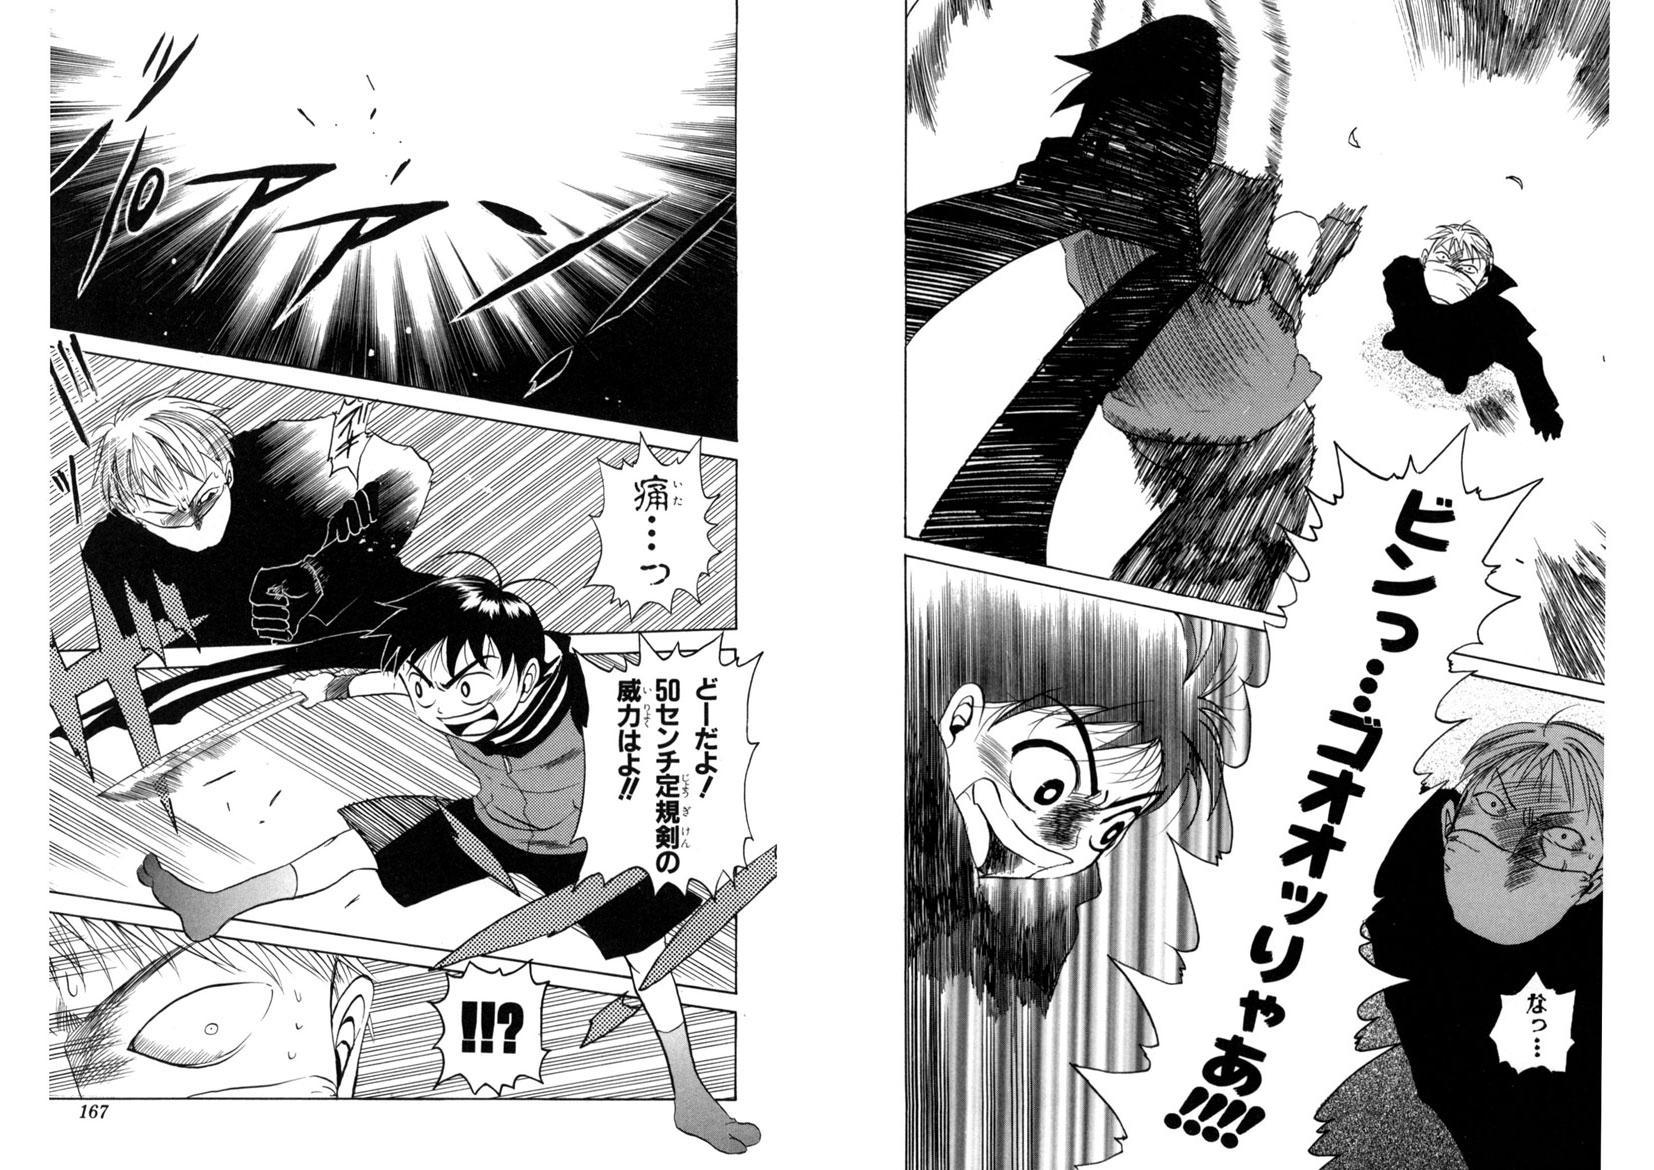
\includegraphics[width=0.8\textwidth]{pict/05/samples_manga.jpg}
   \caption{本節で例示する Manga109NameDataset の入力見開き画像(漫画:『	あっけら貫刃帖』©小林 ゆき/集英社)．}
   \label{fig:sample_manga}
\end{figure}

\begin{figure}[p]
   \centering
   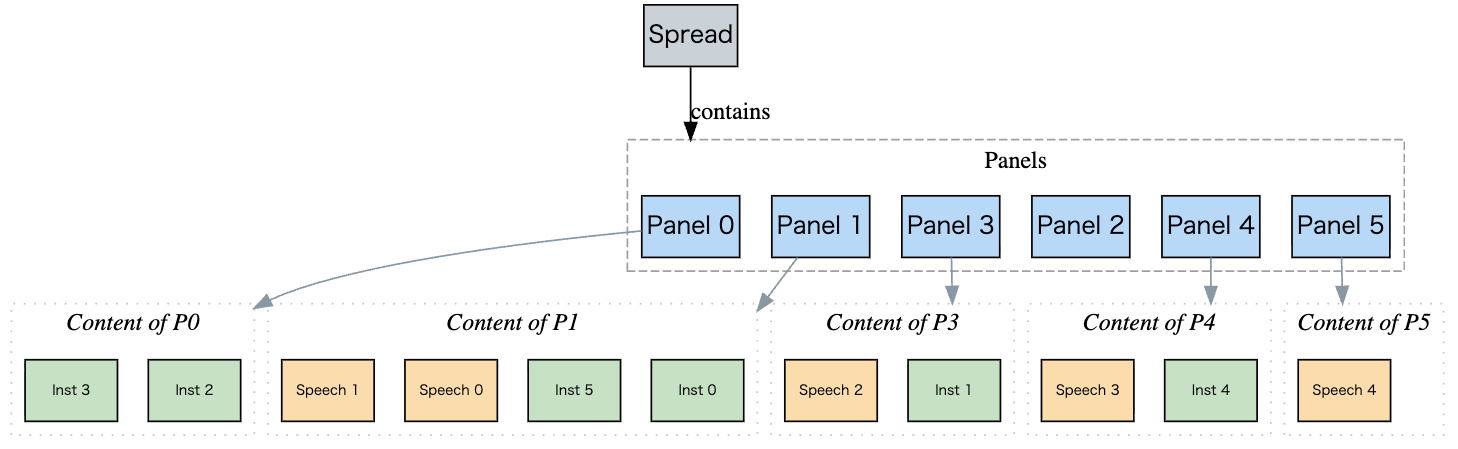
\includegraphics[width=\textwidth]{pict/05/samples_hierarcny.png}
   \caption{構築された階層構造の例．InstはCharacterInstanceノードを表す．}
   \label{fig:sample_hierarchy}
\end{figure}

\begin{figure}[p]
   \centering
   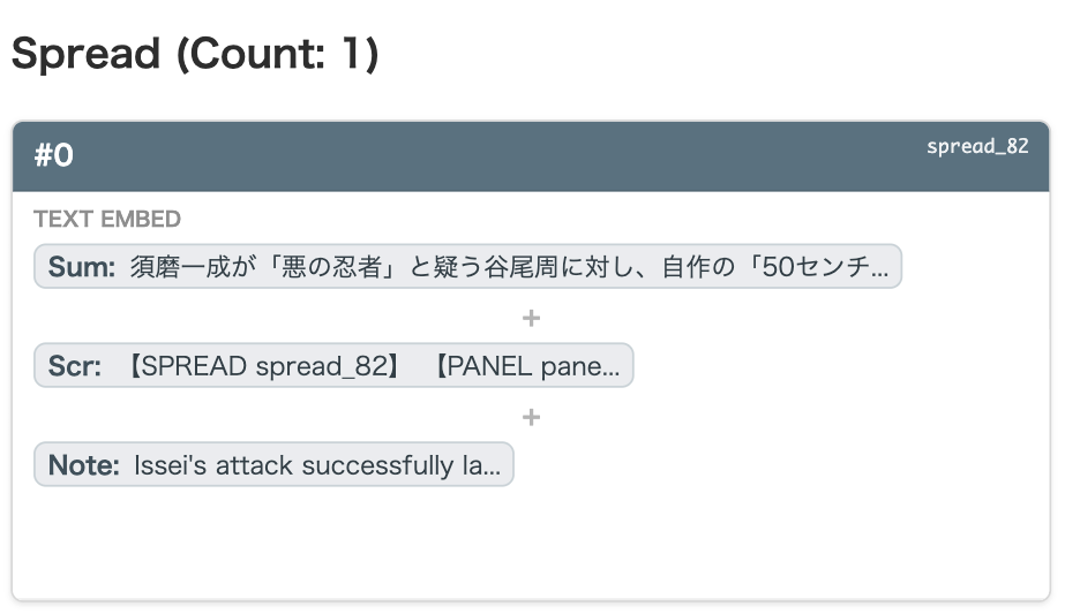
\includegraphics[width=0.60\textwidth]{pict/05/samples_spread.png}
   \caption{Spread ノードの例．}
   \label{fig:sample_spread}
\end{figure}

\begin{figure}[p]
   \centering
   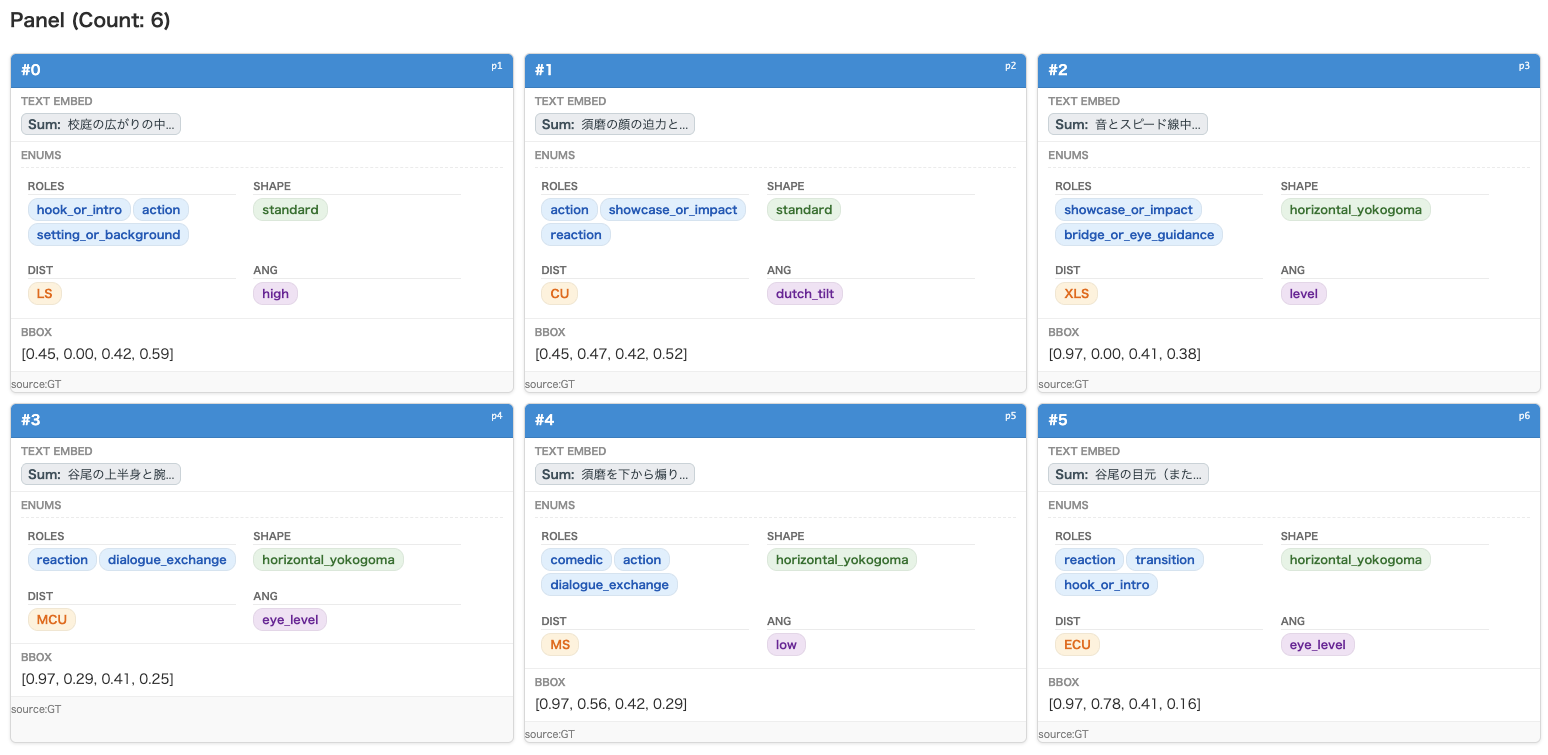
\includegraphics[width=\textwidth]{pict/05/samples_panels.png}
   \caption{Panel ノードの例．}
   \label{fig:sample_panels}
\end{figure}

\begin{figure}[p]
   \centering
   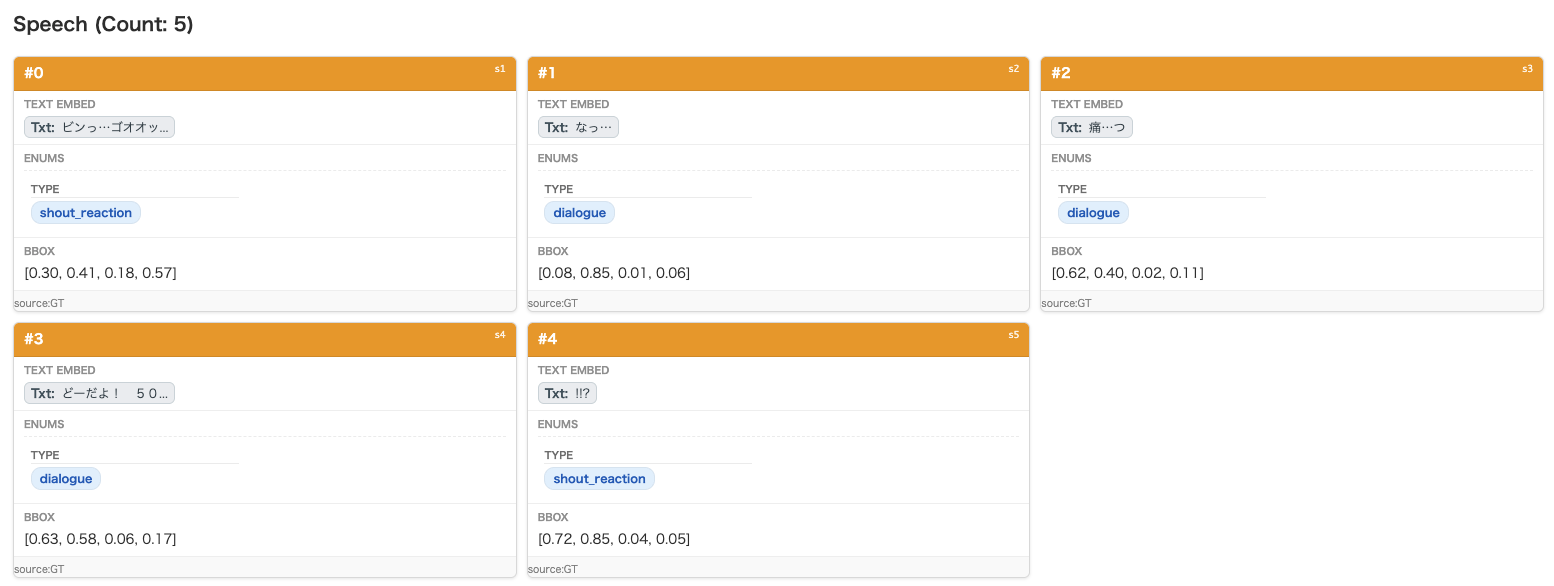
\includegraphics[width=\textwidth]{pict/05/samples_speech.png}
   \caption{Speech ノードにの例．}
   \label{fig:sample_speech}
\end{figure}

\begin{figure}[p]
   \centering
   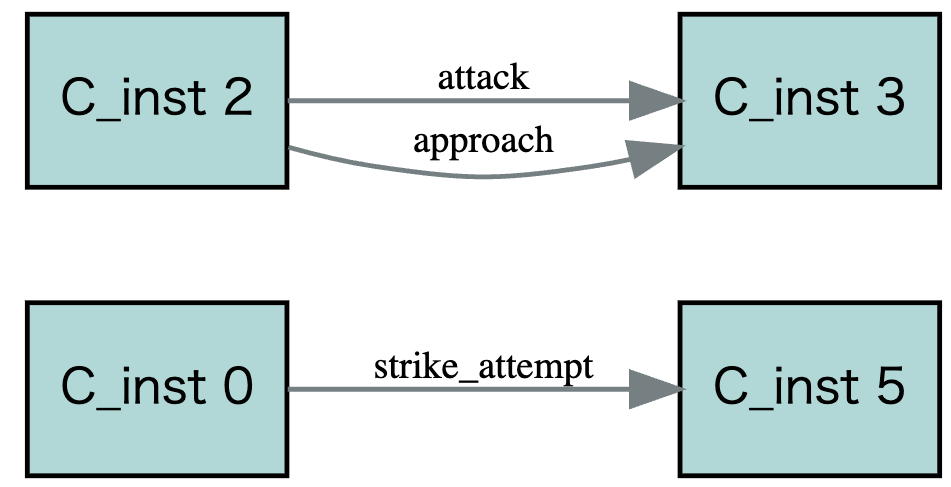
\includegraphics[width=0.50\textwidth]{pict/05/samples_action_edge.png}
   \caption{キャラクターインスタンス間の相互作用（Action Edge）の例．C\_instはCharacterInstanceノードを表す．}
   \label{fig:sample_action_edge}
\end{figure}
\begin{figure}[p]
   \centering
   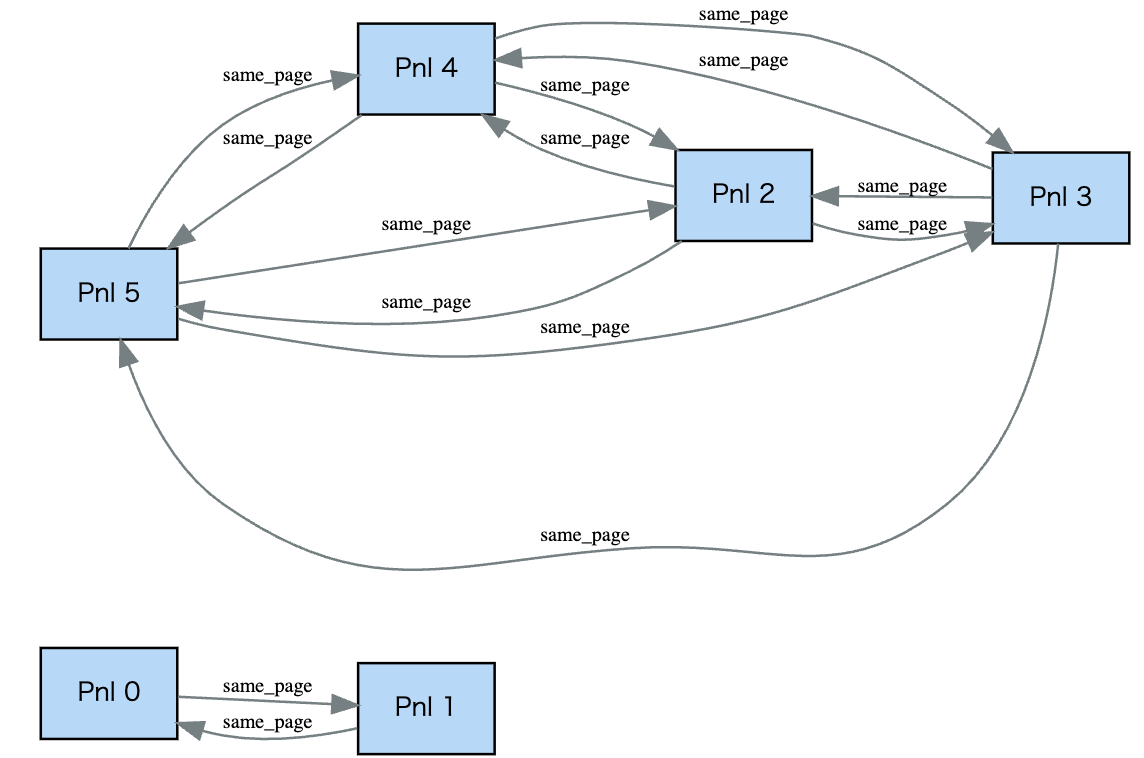
\includegraphics[width=\textwidth]{pict/05/samples_samepages.png}
   \caption{同一ページ内のPanel間の参照関係の例．PnlはPanelノードを表す．}
   \label{fig:sample_samepages}
\end{figure}
\begin{figure}[p]
   \centering
   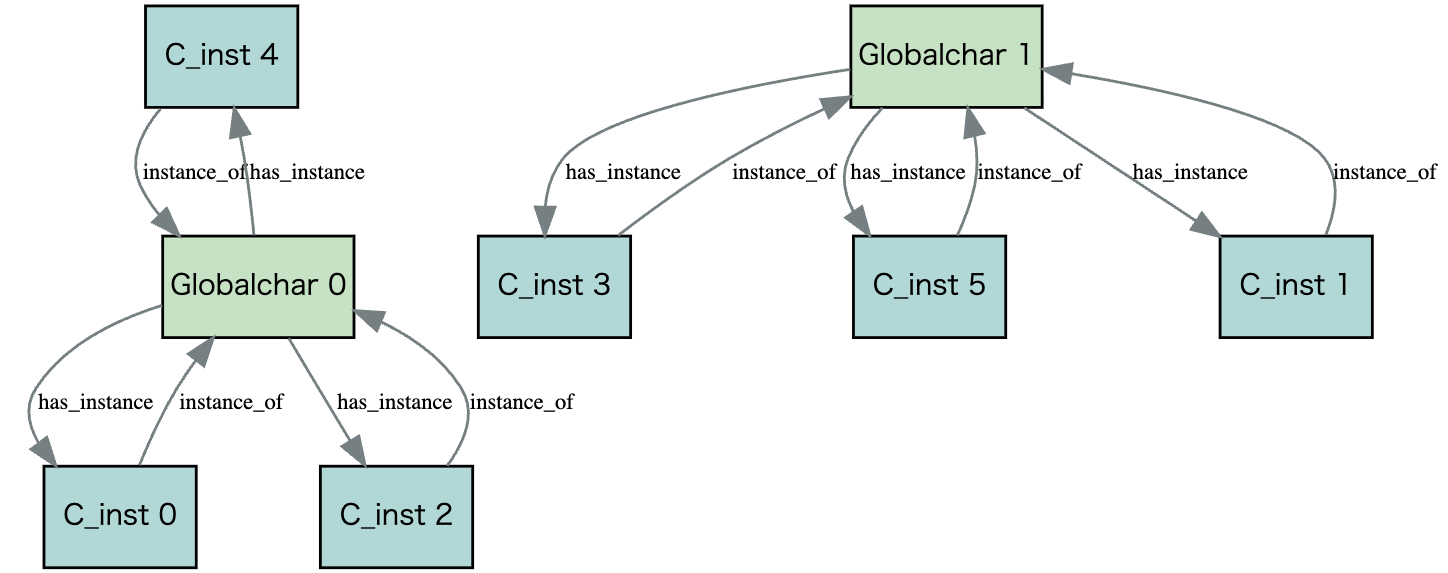
\includegraphics[width=\textwidth]{pict/05/samples_character_edge.png}
   \caption{CharacterInstanceとCharacterNode間の参照関係の例．C\_instはCharacterInstanceノードを表し，GlobalcharはCharacterノードを表す．}
   \label{fig:sample_character_edge}
\end{figure}
\begin{figure}[p]
   \centering
   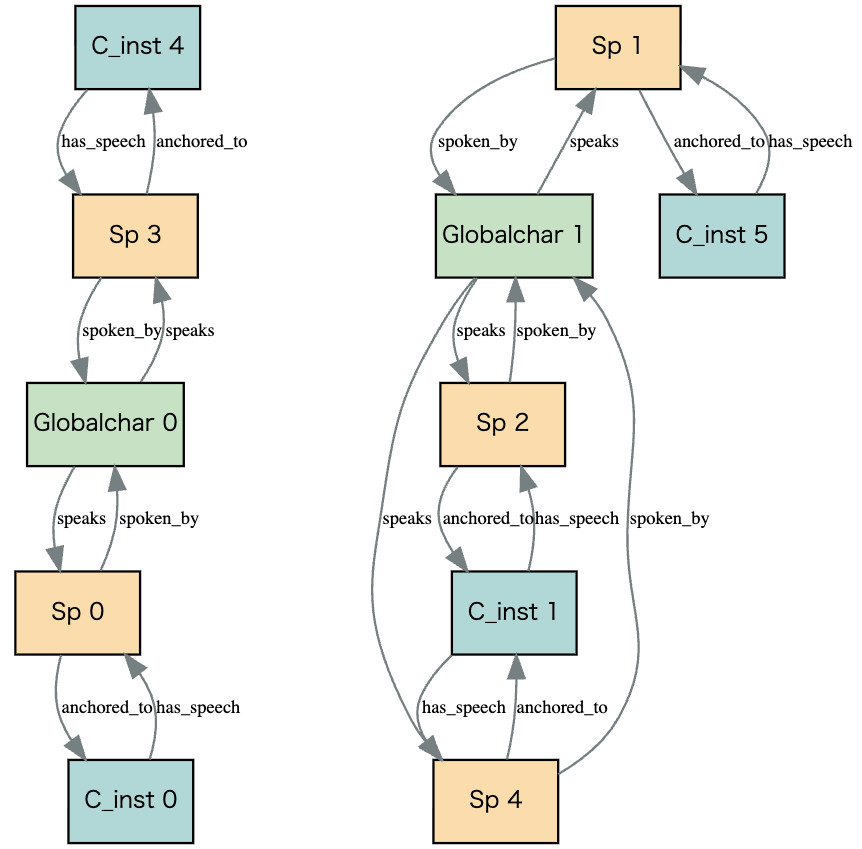
\includegraphics[width=0.7\textwidth]{pict/05/samples_speech_edge.png}
   \caption{SpeechとCharacter Instance および Character を結ぶ参照関係の例．C\_instはCharacterInstanceノードを表し，SpはSpeechノードを，GlobalcharはCharacterノードを表す．}
   \label{fig:sample_speech_edge}
\end{figure}

% ▼▼▼ 仕掛け：main じゃないとき（単体のとき）だけ参考文献を表示 ▼▼▼
\ifdefined\ismain\else
   \printbibliography[title=参考文献]
\fi
% ▲▲▲▲▲▲▲▲▲▲▲▲▲▲▲▲▲▲▲▲▲▲▲▲▲▲▲▲▲▲▲▲▲▲▲▲

\end{document}